% !TeX TXS-program:compile = txs:///pdflatex/[--shell-escape]
% Basado en el template realizado por Diego Essaya, disponible en
%                                                         http://lug.fi.uba.ar
% Modificado por Sebastián Santisi.
% 2007: Modificado por Patricio Moreno y Michel Peterson.
% 2014: Modificado por Patricio Moreno.
% 2017: Modificado por Patricio Moreno.
% 2021: Modificado por Carla Sobico.
% 2024: Modificado(simplificado) por Francisco Del Rio.

% Acá se define el tamaño de letra principal:
% Para utilizar los estilos de KOMA-script, desconectar la línea siguiente y
% comentar la que le sigue (dejar sin comentar un único documentclass)
%\documentclass[10pt, spanish]{scrartcl}
\documentclass[a4paper, twoside, 10pt, spanish]{article}

%%%%%%%%%%%%%%%%%%%%%%%%%%%%%%
% CS
%%%%%%%%%%%%%%%%%%%%%%%%%%%%%%
\usepackage{listings}

\usepackage{booktabs}
\usepackage[margin=1in]{geometry}
\usepackage{array}
\usepackage{pdflscape}
\usepackage{multirow}

% CONFIGURACIONES GENERALES
%%%%%%%%%%%%%%%%%%%%%%%%%%%%%%%%%%%%%%%%%%%%%%%%%%%%%%%%%%%%%%%%%%%%%%%%%%%%%
% Definición del tamaño de página y los márgenes:
% Si preferís menos márgenes, descomentá la línea siguiente
%\usepackage[a4paper,headheight=16pt,scale={0.7,0.8},hoffset=0.5cm]{geometry}
\usepackage[demo]{graphicx}
\usepackage{caption}
\usepackage{subcaption}
\usepackage{babel}  % contiene la correcta separación en sílabas del español
\usepackage[utf8x]{inputenc}    % porque el encoding del documento es UTF-8
\usepackage[per-mode=fraction]{siunitx}
\sisetup%
{
	output-decimal-marker = {,},
	exponent-product = \cdot,
    group-digits = integer,
	group-separator = {.}
}


%
% El paquete amsmath agrega algunas funcionalidades extra a las fórmulas.
% Además defino la numeración de las tablas y figuras al estilo "Figura 2.3",
% en lugar de "Figura 7". (Por lo tanto, aunque no uses fórmulas, si querés
% este tipo de numeración dejá el paquete amsmath descomentado).
%
\usepackage{amsmath, amsfonts, amssymb}
%\numberwithin{equation}{section}
%\numberwithin{figure}{section}
\numberwithin{table}{section}
%%%%%%%%%%%%%%%%%%%%%%%%%%%%%%%%%%%%%%%%%%%%%%%%%%%%%%%%%%%%%%%%%%%%%%%%%%%%%

%%%%%%%%%%%%%%%%%%%%%%%%%%%%%%%%%%%%%%%%%%%%%%%%%%%%%%%%%%%%%%%%%%%%%%%%%%%%%
% ENCABEZADO y PIE DE PÁGINA
%%%%%%%%%%%%%%%%%%%%%%%%%%%%%%%%%%%%%%%%%%%%%%%%%%%%%%%%%%%%%%%%%%%%%%%%%%%%%
\usepackage{fancyhdr}   % Para poder personalizarlo
\usepackage{lastpage}   % Para poder saber cuántas páginas tiene el documento
\pagestyle{fancy}
\renewcommand{\sectionmark}[1]{\markboth{}{\thesection\ \ #1}}
\fancyhead{}	% Elimino el contenido del encabezado
% Muestra la sección a la derecha (izquierda) en páginas impares (pares)
\fancyhead[RO,LE]{\rightmark}
% El siguiente texto a la derecha (izquierda) en páginas pares (impares)
\fancyhead[RE,LO]{TA138 - Entrega final}
\fancyfoot{}	% Elimino el contenido del pie de página
% A la izquierda (derecha) en páginas pares (impares): nro. de página / total
\fancyfoot[LE,RO]{\thepage/\pageref{LastPage}}
%%%%%%%%%%%%%%%%%%%%%%%%%%%%%%%%%%%%%%%%%%%%%%%%%%%%%%%%%%%%%%%%%%%%%%%%%%%%%

%%%%%%%%%%%%%%%%%%%%%%%%%%%%%%%%%%%%%%%%%%%%%%%%%%%%%%%%%%%%%%%%%%%%%%%%%%%%%
% Hipervínculos (enlaces) en el documento (y modificación de atributos)
%%%%%%%%%%%%%%%%%%%%%%%%%%%%%%%%%%%%%%%%%%%%%%%%%%%%%%%%%%%%%%%%%%%%%%%%%%%%%
\usepackage{url}
\urlstyle{tt}
\usepackage[colorlinks=true,linkcolor=black, urlcolor=blue]{hyperref}
\hypersetup{
    breaklinks,
    baseurl       = http://,
    pdfborder     = 0 0 0,
    pdfpagemode   = UseNone,
    pdfstartpage  = 1,
    pdfcreator    = {Plantilla de informe de TP para \LaTeX{}},
    bookmarksopen = true,
    bookmarksdepth= 2,% to show sections and subsections
    pdfauthor     = {Apellido~1, Apellido~2, Apellido~3},
    pdftitle      = {-},
    pdfsubject    = {Informe},
    pdfkeywords   = {}%
    }
%%%%%%%%%%%%%%%%%%%%%%%%%%%%%%%%%%%%%%%%%%%%%%%%%%%%%%%%%%%%%%%%%%%%%%%%%%%%%

%%%%%%%%%%%%%%%%%%%%%%%%%%%%%%%%%%%%%%%%%%%%%%%%%%%%%%%%%%%%%%%%%%%%%%%%%%%%%
% LISTAS (para poder modificar los 'bullets' de las listas)
%%%%%%%%%%%%%%%%%%%%%%%%%%%%%%%%%%%%%%%%%%%%%%%%%%%%%%%%%%%%%%%%%%%%%%%%%%%%%
\usepackage{enumerate}
%%%%%%%%%%%%%%%%%%%%%%%%%%%%%%%%%%%%%%%%%%%%%%%%%%%%%%%%%%%%%%%%%%%%%%%%%%%%%

%%%%%%%%%%%%%%%%%%%%%%%%%%%%%%%%%%%%%%%%%%%%%%%%%%%%%%%%%%%%%%%%%%%%%%%%%%%%%
% TABLAS (para que se vean bien)
%%%%%%%%%%%%%%%%%%%%%%%%%%%%%%%%%%%%%%%%%%%%%%%%%%%%%%%%%%%%%%%%%%%%%%%%%%%%%
\usepackage{booktabs}
\usepackage{multirow}
\usepackage{makecell}
%%%%%%%%%%%%%%%%%%%%%%%%%%%%%%%%%%%%%%%%%%%%%%%%%%%%%%%%%%%%%%%%%%%%%%%%%%%%%

%%%%%%%%%%%%%%%%%%%%%%%%%%%%%%%%%%%%%%%%%%%%%%%%%%%%%%%%%%%%%%%%%%%%%%%%%%%%%
% IMÁGENES
%%%%%%%%%%%%%%%%%%%%%%%%%%%%%%%%%%%%%%%%%%%%%%%%%%%%%%%%%%%%%%%%%%%%%%%%%%%%%
% Para incluir imágenes, el siguiente código carga el paquete graphicx
% según se esté generando un archivo dvi o un pdf (con pdflatex).

% Para generar dvi, descomentá la linea siguiente:
%\usepackage[dvips]{graphicx}

% Para generar pdf, descomentá las dos lineas seguientes:
\usepackage{graphicx}
\pdfcompresslevel=9

% Todas las imágenes están en el directorio imgs:
\newcommand{\imgdir}{imgs}
\graphicspath{{\imgdir/}}
%%%%%%%%%%%%%%%%%%%%%%%%%%%%%%%%%%%%%%%%%%%%%%%%%%%%%%%%%%%%%%%%%%%%%%%%%%%%%

%%%%%%%%%%%%%%%%%%%%%%%%%%%%%%%%%%%%%%%%%%%%%%%%%%%%%%%%%%%%%%%%%%%%%%%%%%%%%
% DIAGRAMAS DE FLUJO EN DIA
%%%%%%%%%%%%%%%%%%%%%%%%%%%%%%%%%%%%%%%%%%%%%%%%%%%%%%%%%%%%%%%%%%%%%%%%%%%%%
% Necesitas este paquete si haces los diagramas de flujo en el programa Dia
% y exportás a latex
%\usepackage{tikz}
%%%%%%%%%%%%%%%%%%%%%%%%%%%%%%%%%%%%%%%%%%%%%%%%%%%%%%%%%%%%%%%%%%%%%%%%%%%%%

%%%%%%%%%%%%%%%%%%%%%%%%%%%%%%%%%%%%%%%%%%%%%%%%%%%%%%%%%%%%%%%%%%%%%%%%%%%%%
% INSERCIÓN DE CÓDIGO FUENTE
%%%%%%%%%%%%%%%%%%%%%%%%%%%%%%%%%%%%%%%%%%%%%%%%%%%%%%%%%%%%%%%%%%%%%%%%%%%%%
% El paquete recomendado actualmente es minted.
% Documentación: https://www.ctan.org/pkg/minted
%\usepackage[
%        section,    % Numera el código según la sección
%    ]{minted}
% minted provee los comandos:
% 1)  \mint[<opciones>]{<lenguaje>}<delimitador><código><delimitador>
% 2)  \mintinline[<opciones>]{<lenguaje>}<delimitador><código><delimitador>
% 3)  \inputminted[<opciones>]{<lenguaje>}{<archivo>}
%\setminted[c]{
%        style=,
%        linenos,            % Mostrar los números de línea
%        numberfirstline,    % Numerar SIEMPRE la primera línea mostrada
%        tabsize=4,          % Reemplazar las tabulaciones por 4 espacios
%        autogobble          % Eliminar espacio sobrante al comienzo
%    }
%%%%%%%%%%%%%%%%%%%%%%%%%%%%%%%%%%%%%%%%%%%%%%%%%%%%%%%%%%%%%%%%%%%%%%%%%%%%%
% COMANDOS UTILES
%%%%%%%%%%%%%%%%%%%%%%%%%%%%%%%%%%%%%%%%%%%%%%%%%%%%%%%%%%%%%%%%%%%%%%%%%%%%%
% los siguientes comandos permiten escribir de manera uniforme en todo el
% documento

% Para poder manejar los espacios al final de los comandos propios
\usepackage{xspace}

% Abreviatura de 'número' utilizando letras voladas (correcto español)
\newcommand{\Nro}{N.\textsuperscript{o}\xspace}
\newcommand{\nro}{n.\textsuperscript{o}\xspace}
%%%%%%%%%%%%%%%%%%%%%%%%%%%%%%%%%%%%%%%%%%%%%%%%%%%%%%%%%%%%%%%%%%%%%%%%%%%%%
% PAQUETES EXTRAS
%%%%%%%%%%%%%%%%%%%%%%%%%%%%%%%%%%%%%%%%%%%%%%%%%%%%%%%%%%%%%%%%%%%%%%%%%%%%%
\usepackage{circuitikz}
\usepackage{float}
\usepackage{multicol}
%\usepackage{pdfpages}
%\usepackage{subfigure}
%\usepackage{graphicx}%
\usepackage{gensymb}
\usepackage{titlesec}

\setcounter{secnumdepth}{4}

\titleformat{\paragraph}
{\normalfont\normalsize\bfseries}{\theparagraph}{1em}{}
\titlespacing*{\paragraph}
{0pt}{3.25ex plus 1ex minus .2ex}{1.5ex plus .2ex}

%%%%%%%%%%%%%%%%%%%%%%%%%%%%%%%%%%%%%%%%%%%%%%%%%%%%%%%%%%%%%%%%%%%%%%%%%%%%%
%%%%%%%%%%%%%%%%%%%%%%%%%%%%%%%%%%%%%%%%%%%%%%%%%%%%%%%%%%%%%%%%%%%%%%%%%%%%%
% INICIO DEL DOCUMENTO
%%%%%%%%%%%%%%%%%%%%%%%%%%%%%%%%%%%%%%%%%%%%%%%%%%%%%%%%%%%%%%%%%%%%%%%%%%%%%
%%%%%%%%%%%%%%%%%%%%%%%%%%%%%%%%%%%%%%%%%%%%%%%%%%%%%%%%%%%%%%%%%%%%%%%%%%%%%
\begin{document}


%
% Carátula:
%
\begin{titlepage}

\thispagestyle{empty}

\begin{center}
\includegraphics[scale=0.3]{res/fiuba.pdf}\\
\large{\textsc{Universidad de Buenos Aires}}\\
\large{\textsc{Facultad de Ingeniería}}\\
% Modificar año y cuatrimestre
\small{Año 2025 - 2\textsuperscript{o} cuatrimestre}
\end{center}

\vfill

\begin{center} % Modificar el código de ser necesario
\Large{\underline{\textsc{Taller de diseño de circuitos electrónicos (TA138)}}}\\
\vspace{.5cm}
 \Large{\textsc{Entrega final - Sistema de alimentación para aplicaciones industriales y automotrices}}
\end{center}

\vfill

 \begin{tabbing}

	\\\hspace{2cm}\=\+\\ \\
% %	FECHA : DD/MM/2019\\% \today\\
%TUTOR: Lorem ipsum dolor sit amet, \\
 \\
	ESTUDIANTES: Grupo 4\hspace{-1cm}\=\+\hspace{1cm}\=\hspace{6cm}\=\\
            Martin, Andrés	\>\> 110722\\ 
              \>\footnotesize{\verb!ammartin@fi.uba.ar!}\\
            Loñ, Julieta	\>\> 110663\\ 
              \>\footnotesize{\verb!jlon@fi.uba.ar!}\\ 		    
            Monti, Martina	\>\> 110574\\ 
              \>\footnotesize{\verb!mmonti@fi.uba.ar!}\\
            Del Rio, Francisco	\>\> 110761\\ 
              \>\footnotesize{\verb!fadelrio@fi.uba.ar!}\\           
 \end{tabbing}



\vfill

\hrule
\vspace{0.2cm}

% Modificar código de ser necesario
\noindent\small{TA138 - Taller de diseño de circuitos electrónicos \hfill}

\end{titlepage}

%
% Hago que las páginas se comiencen a contar a partir de aquí:
%
\setcounter{page}{1}

%
% Pongo el índice en una página aparte:
%

\tableofcontents
\newpage
%
% Inicio del TP:
%

\section{Primer Checkpoint}

\subsection{Introducción}

\quad En este trabajo se aplicarán los conceptos aprendidos en las clases teóricas. Se observará el comportamiento de distintas fuentes de alimentación lineales. En ellas, apoyados de teoría y pruebas empíricas se lograrán amplias mejoras para el diseño de la fuente. Se partirá de una fuente muy básica, dependiente de la temperatura de los componentes y variaciones de la $V_{IN}$ hasta una fuente capaz de limitar la potencia en casos extremos para no deteriorar los componentes de la fuente.

\subsection{Regulador de Tensión}
\quad Se busca obtener una tensión de salida estable de \SI{5}{V}, que presente poca variación ante grandes variaciones de la tensión de entrada, es decir buena regulación de linea. También se espera que la tensión se mantenga a medida que varía la corriente de salida dentro de cierto rango, es decir que presente una buena regulación de carga. A lo largo de esta sección se explicará el recorrido tomado para obtener estas especificaciones, tanto como qué se considera como ``bueno'' en ambos casos.
%%%%%%%%%%%%%%%%%%%%%%%%%%%%%%%%%%%%%%%%%%%%%%%%%%%%%%%%%%%%%%%%%%%%%%%%%%%%%%%%%%%%%%%%%%%%%%%%%%%%%%%%%%%%%%%%%%%
\subsubsection{Diagrama de bloques}\label{sec:diagrama_de_bloques}
\quad La mejor forma de estabilizar un parámetro de la salida es a través de un muestreo de éste parámetro y su comparación con una referencia, es decir, un sistema realimentado. Para nuestro caso, lo adecuado es muestrear tensión a la salida y sumar tensión a la entrada, de esta forma se acerca nuestro sistema a un amplificador ideal de tensión. 

\begin{figure}[H]
	\centering
	\includegraphics[width=0.7\linewidth]{res/esquema_diagrama_de_bloques.png}
	\caption{Diagrama de bloques de el sistema realimentado}
	\label{fig:esquema_diagrama_de_bloques}
\end{figure}

\quad Como se puede ver en el diagrama de bloques, la entrada al amplificador realimentado es $V_{ref}-V_{of}$, lo que implica realimentación negativa. Realimentando negativamente se consigue estabilizar el parámetro de interés a la salida, ya que si la ganancia de lazo $T = af$ es lo suficientemente grande, se tiene:

$$V_o = \frac{a}{1+af}V_{ref}  \xrightarrow[af\gg1]{} \frac{V_{ref}}{f}$$ 

\quad De esta forma, con un circuito diseñado para obtener la ganancia de lazo necesaria, la tensión de salida dependerá solamente de la referencia y de la realimentación, que en nuestro caso será un simple divisor resistivo.


%%%%%%%%%%%%%%%%%%%%%%%%%%%%%%%%%%%%%%%%%%%%%%%%%%%%%%%%%%%%%%%%%%%%%%%%%%%%%%%%%%%%%%%%%%%%%%%%%%%%%%%%%%%%%%%%%%%
\subsubsection{Elección del transistor de paso}
\quad Se necesita una corriente elevada a la salida, como no todos los transistores pueden controlar altas corrientes, y más adelante, un par diferencial no puede satisfacer por si mismo. La manera de resolver esto fue agregando un buffer de corriente en la forma de un Quasi-Darlington. A diferencia del Darlington el Quasi-Darlington permite que la caída de tensión sobre el transistor de paso sea mas chica, lo cual ayuda a tener un Low-Dropout. 

\quad El transistor de paso es el encargado de dispar la mayor parte de la potencia del circuito por lo tanto al momento de elegirlo se buscaron transistores que puedan disipar la potencia necesaria, y que puedan soportar la corriente y tensión entres sus bornes requerida. La corriente máxima que pasa por el transistor sera \SI{1.5}{A} y la tensión de entrada puede variar entre \SI{9.5}{V} y \SI{24}{V}, usando esa información calculamos la potencia máxima como $P_{max} = I_{max}(Vin_{max}- \SI{5}{V}) = $ \SI{28.5}{W}

\quad El valor de la ganancia de corriente también fue relevante en la elección, es necesario que esta no disminuya demasiado a altas corrientes. Este fue uno de los requisitos mas restrictivos ya que varias de las opciones disponibles cuando operan a \SI{1.5}{A} presentan una ganancia de corriente cercana a 10. 

\quad Finalmente, la mayor limitación estuvo dada por la disponibilidad de los componentes en las casas de electrónica cercanas. Y en caso de que este disponible, el precio también se tuvo en cuenta. Se considero que el transistor elegido debía ser accesible de manera que se puedan comprar en cantidad y reemplazarlo en caso de ser necesario. 

\quad En base a todo lo mencionado se eligió el transistor \textbf{MJE2955T} que cumple con todas las características mencionadas. Las necesidades de corriente, tensión y potencia son cubiertas por un gran margen. La variación de la ganancia de corriente se puede ver en el gráfico \ref{fig:datasheet_hfe}, en la corriente de operación presenta un valor cercano a 70.
%ACA FOTITO DEL GRAFICO DE BETA PLISSSSSSSSSSSSSSSSSSSSSSSSSSSSSSSSSSSSSSSSSSSSSSSSSSSSSS referencia grafico_beta

\begin{figure}[H]
	\centering
	\includegraphics[width=0.6\linewidth]{res/datasheet_hfe.png}
	\caption{Caption}
	\label{fig:datasheet_hfe}
\end{figure}

\quad El transistor de drive usado sera el \textbf{BC547}. Se seleccionó este transistor debido a que tiene una ganancia lo suficientemente alta y a la disponibilidad del modelo ya que es el mismo que sera utilizado para otros transistores presentes en el circuito. 



%%%%%%%%%%%%%%%%%%%%%%%%%%%%%%%%%%%%%%%%%%%%%%%%%%%%%%%%%%%%%%%%%%%%%%%%%%%%%%%%%%%%%%%%%%%%%%%%%%%%%%%%%%%%%%%%%%%
\subsubsection{Primer diseño}

\begin{figure}[H]
	\centering
	\includegraphics[width=0.7\linewidth]{res/esquema_primer_circuito.png}
	\caption{Primer diseño de regulador lineal de tensión}
	\label{fig:esquema_primer_circuito}
\end{figure}

\quad Como primer diseño, se utilizó el circuito presentado en la figura \ref{fig:esquema_primer_circuito} el cual tiene ciertas limitaciones en comparación con el diseño final. En el gráfico de la \autoref{fig:graf_reglin_primer}, de regulación de linea se ve que hay una gran variación de la tensión de salida con respecto a variaciones de la tensión de entrada, obteniendo una variación de $\SI{23.6}{\frac{mV}{V}}$ y en el gráfico de la \autoref{fig:graf_regcar_primer}, de regulación de carga se puede apreciar la variación que tiene la tensión de salida frente a modificaciones del valor de la $R_{carga}$, obteniendo un valor de regulación de carga de \SI{358}{m\ohm}. Lo que se busca es lograr que la tensión de salida quede lo más estable posible en 5V independientemente del valor que tome la $R_{carga}$ y de las variaciones qué puede presentar $V_{in}$ por lo que el $\Delta V_{sal}$ con respecto a estas variables se quiere reducir lo mayor posible, y este modelo no cumple con este requerimiento. 

\quad Otro problema que presenta este modelo es que las variaciones de $V_{be}$ forman parte de la tensión de referencia, lo cual provoca que frente a variaciones en por ejemplo la temperatura, la $V_{ref}$ cambie su valor, cambiando así también el valor de la tensión de salida puesto que $V_{salida}$ = $\frac{a}{1+T}$ * $V_{ref}$

\quad Realizando la simulación de la ganancia de lazo se observa un valor de 30 veces. Esta simulación se realizó añadiendo un inductor entre $R_{f2}$ y $R_l$ (en el nodo de $R_{f2}$), un capacitor entre $R_{f2}$ y el inductor, y una fuente de tensión alterna que conecta a este capacitor con tierra. Teniendo en cuenta la ecuación de la \autoref{sec:diagrama_de_bloques}, la ganancia de lazo resulta, en cierta medida, comparable con 1, lo que explica el pobre desempeño en regulación de carga y linea. Esta ganancia es mejorable y esto se apreciará mejor en la comparación de la ganancia de lazo del par diferencial.

\begin{figure}[H]
	\centering
	\includegraphics[width=1\linewidth]{res/graf_reglin_primer.jpeg}
	\caption{Regulación de linea del diseño}
	\label{fig:graf_reglin_primer}
\end{figure}

\begin{figure}[H]
	\centering
	\includegraphics[width=1\linewidth]{res/graf_regcar_primer.jpeg}
	\caption{Regulación de carga del diseño}
	\label{fig:graf_regcar_primer}
\end{figure}

\subsubsection{Diseño con par diferencial}
Con el motivo de mejorar la regulación del circuito, disminuyendo las variaciones de $V_{sal}$ con respecto a la $R_{carga}$ y a $V_{in}$, se modificó el circuito de entrada con par diferencial permitiendo así tener un mejor rechazo en modo común y una mayor ganancia de lazo del sistema. También, se colocaron resistencias de 100 $\ohm$ en el emisor de la carga activa, estas sirven para arreglar futuros desapareamientos que podrían presentarse.

\quad Al colorarle al par diferencial la carga activa, se ayuda a mejorar el rechazo de modo común, disminuyendo la ganancia del respectivo modo y a su vez aumentando el RRMC. 

\quad Además, al usar un amplificador diferencial se consigue independizar la referencia de valores intrínsecos de los transistores, como la tensión base-emisor, que presentan altas variaciones con temperatura y otros parámetros.  


\begin{figure}[H]
	\centering
	\includegraphics[width=\linewidth]{res/esquema_circuito_con_par_bloques.pdf}
	\caption{Diseño con amplificador diferencial}
	\label{fig:esquema_circuito_con_par_diferencial}
\end{figure}

\quad Como se puede ver en los bloques del circuito, la tensión de entrada al amplificador diferencial es $V_{Ref} - V_{oR}$, entonces la referencia de la realimentación depende solamente de la tensión $V_{ref}$, que más adelante se especificará cómo esta se puede obtener asegurando poca variación ante parámetros tanto externos como internos al circuito.

\quad Si se compara la regulación de carga del primer diseño con el del par diferencial, se ve que el valor con este último circuito es más de 100 veces menor que el valor que se obtuvo con el primero diseño lo cual indica que nuestra $V_{out}$ tiene menores variaciones en función de la carga.

\quad Además gracias a la carga activa el circuito tendrá un mayor rechazo de modo común por lo que se tendrá una mayor ganancia.

\begin{figure}[H]
	\centering
	\includegraphics[width=1\linewidth]{res/graf_regcar_par.jpeg}
	\caption{Regulación de carga del diseño con par diferencial}
	\label{fig:graf_regcar_par}
\end{figure}


\quad También está el gráfico de regulación de línea en el cual, comparando con el primer diseño, su valor corresponde a \SI{23.6}{mV} y en el diseño actual a \SI{2.86}{mV}. Esta disminución de su valor indica que la $V_{out}$ del diseño final presenta alrededor de 10 veces menos variaciones en función de la $V_{in}$ respecto al primer diseño. 



\begin{figure}[H]
	\centering
	\includegraphics[width=1\linewidth]{res/graf_reglin_par.jpeg}
	\caption{Regulación de linea del diseño con par diferencial}
	\label{fig:graf_reglin_par}
\end{figure}

\quad Ademas se calculó la ganancia de lazo, cortando el lazo en la base de Q2, dado que la resistencia de entrada al par diferencial es de aproximadamente \SI{25}{K\ohm}, entonces su efecto junto a la red de realimentación en la carga es despreciable. Se obtuvo un valor aproximado de T de 1000 veces. Luego se simuló esta misma y se obtuvo un valor de 708 veces, lo que implica un error de cálculos de aproximadamente un 30\%. Tal error puede atribuirse a la nula disponibilidad de valores de parámetros intrínsecos de los transistores, como son la tensión de early o la ganancia de corriente, la cual presenta gran dispersión.

\quad Aún con el error de cálculos, los valores obtenidos son lo suficientemente mayores a 1 como para que la ganancia del sistema realimentado se pueda considerar $\frac{V_{ref}}{f}$ lo que, como se puede ver en los gráficos de regulación de linea y carga de las figuras \ref{fig:graf_regcar_par} y \ref{fig:graf_reglin_par} resulta en un parámetro mucho más estable a la salida ante variaciones de tensión de entrada y corriente de salida.


\paragraph{Polarización del par diferencial con fuente de corriente}


\quad Para mejorar el rechazo de modo común y dejar una corriente fija para la polarización del circuito, se coloca una fuente de corriente polarizada con la misma tensión de referencia de la base de Q1, en el emisor del par. En el análisis para modo diferencial, ese punto es una tierra virtual por lo que no modifica la ganancia en ese modo pero, en modo común agregar la fuente de corriente, que presenta un alto valor de resistencia en los emisores del par, deriva en que la ganancia del modo común disminuya y por lo tanto que la RRMC aumente. 


\subsection{Limite de corriente}


\quad Al momento de hacer una fuente de alimentación hay que considerar todos los casos. Si no se coloca ningún limitador el circuito se podría dañar frente a diferentes situaciones; ya sea demasiada potencia requerida, cortocircuito, entre otros. 

\begin{figure}[H]
	\centering
	\includegraphics[width=0.8\linewidth]{res/esquema_reg_corriente.png}
	\caption{Circuito con regulador de corriente}
	\label{fig:esquema_reg_corriente}
\end{figure}

\quad En este circuito se observa que se utiliza un transistor BC547C un resistor de \SI{0.42}{\ohm} para crear un lazo de realimentación en el circuito. El transistor esta conectado de manera tal que cuando aparezca una caída de \SI{0.63}{V} en la resistencia previamente nombrada, se activa Q7. Notar que que \SI{0.63}{V} con una resistencia de \SI{0.42}{\ohm} equivale a una corriente de \SI{1.5}{A}, exactamente la corriente que queremos limitar. De esta forma, cumpliendo la Ley de corrientes de Kircchoff Q3 deja de recibir toda la corriente de la etapa anterior y un porcentaje de esa corriente lo toma Q7. Esto genera que el driver (Q3) del darlington no amplifique como antes y la corriente total que recibe la carga se mantiene en \SI{1.5}{A}. 

%\quad Cabe resaltar que este efecto se genera con continuas variaciones. Cuando Q7 toma corriente, por Rs baja la corriente y por lo tanto Q7 se apaga. Luego vuelven a circular \SI{1.5}{A} en Rs y vuelve a prenderse Q7 para estabilizar una vez más la corriente. Este ciclo se cumple continuamente hasta que baje la corriente pedida.

\pagebreak

\subsubsection{Limite de corriente por foldback}
Al llegar a la situación dónde circula la corriente máxima, el circuito de la sección anterior limita la corriente pero el transistor de paso está siendo constantemente exigido, ya que entre su colector y emisor circulan \SI{1.5}{A} y cae toda la tensión de entrada, por lo que la potencia disipada en éste transistor es máxima, y la no haber carga, no hay potencia aprovechada a la salida. Para evitar esto se utiliza otro limitador de corriente llamado Foldback. Este permite que, frente a la $V_{salmin}$, el limitador de corriente hará que la corriente que circule por el transistor Q6 no sea \SI{1.5}{A} y sea $I_{cc} = \SI{400}{mA}$. Este método funciona agregando al limitador original de la sección 3 un divisor resistivo el cual genera que el circuito se comporte (únicamente en la sección de foldback) según la siguiente ecuación:
\begin{equation}
	I_{SAL} = \frac{{(R_1 + R_2) * V_{BE}} + R_1 * V_{SAL}}{R_S * R_2}
\end{equation}
\quad Se observa que hay una relación lineal entre $I_S$ Y $V_s$, la cuál corresponde a la forma característica del limitador de corriente por foldback

\begin{figure}[H]
	\centering
	\includegraphics[width=0.8\linewidth]{res/esquema_foldback.png}
	\caption{Circuito con regulador de corriente foldback}
	\label{fig:esquema_foldback}
\end{figure}

\quad En el apéndice se puede ver el detalle de los cálculos utilizados para obtener los valores de las resistencias presentes el el bloque de foldback.

\quad Luego, se simuló el circuito con la implementación del foldback, variando la carga a tensión de entrada constante, y se obtuvo la siguiente curva de corriente de salida contra tensión de salida:

\begin{figure}[H]
	\centering
	\includegraphics[width=\linewidth]{res/graf_foldback.jpeg}
	\caption{Curva de foldback}
	\label{fig:graf_foldback}
\end{figure}

\quad Se puede apreciar como, al disminuir $R_{carga} = \frac{V_o}{I_o}$, la corriente llega hasta un máximo de aproximadamente \SI{1.5}{A} y luego, al acercarse $R_{carga}$ a cero, la corriente disminuye hasta aproximadamente \SI{400}{mA}, disminuyendo la potencia disipada en el transistor de paso al cortocircuitar la salida.

\subsection{Diseño final y esquemático del PCB}

\begin{figure}[H]
	\centering
	\includegraphics[width=0.82\linewidth]{res/diagrama_kicad.png}
	\caption{Esquemático del circuito en KiCad}
	\label{fig:diagrama_kicad}
\end{figure}

\quad El valor de la resistencia que acompaña a la referencia fue elegido en base a la corriente necesaria para alimentar el circuito. Hacia la base del transistor Q1 la corriente es del orden del $\mu$A por lo tanto es despreciable y solo es necesario considerar la de la referencia. En la datasheet del TL431D para la configuración usada, se indica que la corriente puede variar entre \SI{0.5}{mA} y \SI{100}{mA} por lo tanto elige una resistencia de \SI{1}{K\ohm} que es un valor estándar y permite una corriente dentro de la permitida. 

\quad Por otro lado, las resistencias en la carga activa del par permiten corregir desapareamientos entre las ramas, su valor deberá ser modificado luego de medir dichas diferencias de manera que se compensen. No debe ser un valor elevado ya que si tienen una caída muy grande, el par se podría meter en zona de corte. 

\subsubsection{Eficiencia}

\quad Manteniendo la tensión de entrada constante en \SI{9.5}{V}, se calculó la eficiencia para distintas corrientes de salida y se obtuvo el siguiente gráfico:

\begin{figure}[H]
	\centering
	\includegraphics[width=.9\linewidth]{res/graf_eficiencia.jpeg}
	\caption{Eficiencia contra corriente de salida}
	\label{fig:graf_eficiencia}
\end{figure}

\quad Como se puede ver, el gráfico tiene una forma similar al de la \autoref{fig:graf_foldback}, esto se debe a que cuando el comportamiento del circuito está dado por el foldback, la potencia disipada en la carga tiende a cero, hasta finalmente ser cero cuando la carga es un cortocircuito. Luego, la eficiencia para la zona de funcionamiento normal del regulador es levemente mayor al 50\%, lo cual resulta esperable, ya que en esa zona la eficiencia viene principalmente dada por la tensión de entrada al regulador, si la tensión de entrada se encontrara más cerca del limite superior la eficiencia sería mucho menor. Otra zona de interés es lo que ocurre a bajas corrientes de salida, ya que al disminuir la corriente de salida, esta se vuelve comparable con las corrientes de polarización del par diferencial y la referencia de tensión, que si bien son corrientes bajas y por lo tanto potencias disipadas bajas, comparadas con la potencia casi nula sobre la carga, hacen que la eficiencia tienda a cero.

\subsection{Conclusiones}
%%%%%%%%%%%%%%%%%%%%%%%%%%%%%%%%%%%%%%%%%%%%%%%%%%%%%%%%%%%%%%%%%%%%%%%%%%%%%%%%%%%%%%%%%%%%%%%%%%%%%%%%%%%%%%%%%%%
\quad Los resultados obtenidos en este trabajo cumplen con lo esperado.
Se logro obtener una regulación de linea y de carga con bajos valores, y la implementación de la regulación por foldback fue exitosa permitiendo limitar la corriente entre $I_{max}$ y $I_{cc}$.

\quad Como cierre de este trabajo, nos llevamos el aprendizaje de buscar no solo que un circuito funcione sino que también sea eficiente. La oportunidad de aplicar temas vistos en materias anteriores en un circuito funcional permitió profundizar en nuestros aprendizajes, practicas y  criterio.

\quad Se experimentó con el diseño y utilizando la teoría vista junto con simulaciones, se llegó un circuito eficiente y que cumple con los requisitos pedidos. 


\subsection{Apéndice}
\quad Para calcular el valor de las resistencias del circuito de foldback inicialmente se plantea la malla que contiene el $V_{be7}$.
\begin{equation}
	V_{be7} = V_{R_s} - V_{R_4} = R_s I_s - (V_o +R_sI_o) \frac{R_4}{R_4 +R_5}
\end{equation}
\quad Si se despeja $I_o$ 
\begin{equation}
	I_o = \frac{V_{be}}{R_s}(1+\frac{R_4}{R_5}) + \frac{V_oR_4}{R_s R_5}
\end{equation}
\quad Cuando $V_o = 0$, se obtiene $I_{cc}$
\begin{equation} \label{eq:Icc}
	Icc = \frac{V_{beON}}{R_s}(1+\frac{R_4}{R_5})
\end{equation}
\quad Considerando que se quiere operar a una corriente máxima de $I_o = 1.5 A$ por lo que la cuenta se limita teniendo en cuenta esa $I_{max}$
\begin{equation}\label{eq:Imax}
	I_{max} = \frac{V_{beON}}{R_s} (1+\frac{R_4}{R_5}) +\frac{V_oR_4}{R_sR_5}
\end{equation}
\quad Luego, se dividen \ref{eq:Imax} y \ref{eq:Icc} para obtener una relación entre $R_4$ y $R_5$.
\begin{equation}
	\frac{I_{max}}{I_{cc}} = 1 + \frac{V_o}{V_{BEON}}\frac{\frac{R_4}{R_5}}{1+\frac{R_4}{R_5}}
\end{equation}
\begin{equation}
	\frac{I_{max}}{I_{cc}} = 1+\frac{V_o}{V_{BEON}}\frac{1}{1+\frac{R_5}{R_4}}
\end{equation}
\begin{equation}\label{eq:R5/R4}
	\frac{R_5}{R_4} = \frac{V_o}{(\frac{I_{max}}{I_{cc}}-1)V_{BEON}}-1
\end{equation}
\quad Luego se despeja $R_{s}$ de \ref{eq:Icc} y se reemplaza usando \ref{eq:R5/R4} para obtener su valor
\begin{equation}
	R_s = \frac{V_{BEON}}{I_{cc}}(1+\frac{R_4}{R_5})
\end{equation}

\newpage

\section{Segundo checkpoint}

\subsection{Introducción}

\quad Esta entrega se centrará en el análisis en frecuencia para el circuito presentado en la entrega anterior. El principal objetivo es asegurar la linealidad de la fuente para todas las frecuencias compensando el circuito, buscando así evitar oscilaciones y realimentaciones positivas no deseadas.
%%%%%%%%%%%%%%%%%%%%%%%%%%%%%%%%%%%%%%%%%%%%%%%%%%%%%%%%%%%%%%%%%%%%%%%%%%%%%%%%%
\subsection{Compensación}

\subsubsection{Lazo de tensión}

\quad  Analizando el comportamiento de la ganancia de lazo en frecuencia, se puede apreciar en las figuras \ref{fig:lazo_tension_sin_compensar_1u} y \ref{fig:lazo_tension_sin_compensar_15u} que el circuito presenta un margen de fase negativo para los limites de capacidad de carga. El margen de fase negativo implica que existe una frecuencia para la cual la fase se encuentra desplazada $-180\degree$ respecto a la fase inicial y la ganancia es mayor a \SI{0}{dB}, lo que implica que la realimentación se vuelva positiva, resultando en un comportamiento inestable.


\begin{figure}[H] 
	\centering 
	\includegraphics[width=1\linewidth]{res/lazo_tension_sin_compensar_1u.jpeg} 
	\caption{Diagrama de bode de T con capacidad de carga de \SI{1}{\micro F}} 
	\label{fig:lazo_tension_sin_compensar_1u} 
\end{figure}

\vfill

\pagebreak


\begin{figure}[H] 
	\centering 
	\includegraphics[width=1\linewidth]{res/lazo_tension_sin_compensar_15u.jpeg} \caption{Diagrama de bode de T con capacidad de carga de \SI{15}{\micro F}} 
	\label{fig:lazo_tension_sin_compensar_15u} 
\end{figure}

\quad Se optó por usar el método de estabilización mediante corrimiento de polo dominante de la respuesta en frecuencia. Para realizar esto se agrega un capacitor seguido de una resistencia en el nodo dominante, como se puede ver en la \autoref{fig:compensado_sin_valores}. 

%\quad En esa frecuencia, la realimentación del circuito se vuelve positiva y por ende podría oscilar. Este efecto se produce ya que existe una rotación de fase de 180° para valores de $\left| T \right|$ mayores a 1 y es muy peligroso ya que provocaría alinealidad de la fuente. Para evitar este efecto se decidió compensar el circuito. Para ello se debió introducir un capacitor de compensación y una resistencia serie a este a común en el nodo dominante formando el siguiente circuito.

\begin{figure}[H] 
	\centering 
	\includegraphics[width=.8\linewidth]{res/compensado sin valores.jpg} 
	\caption{Esquemático con red de compensación} \label{fig:compensado_sin_valores} 
\end{figure}

\quad Para seleccionar el valor del capacitor y de la resistencia, se analizaron los nodos identificando el dominante y mediante simulación se buscó obtener una respuesta en frecuencia deseada colocando una combinación de valores de R y C que muevan el polo dominante. El capacitor utilizado es de \SI{33}{nF} junto con una resistencia de \SI{100}{\ohm}.

\quad Como se puede ver en las Figuras \ref{fig:lazo_tension_compensado_1u} y \ref{fig:lazo_tension_compensado_15u}, el margen de fase obtenido es, en el mejor caso de $103\degree$ y en el peor caso de $37\degree$. De esta forma, se soluciona la posibilidad de inestabilidad mencionada al principio de la sección ya que, para la frecuencia a la que la fase se encuentra desplazada $-180\degree$ respecto a la fase inicial, la ganancia es mucho menor a \SI{0}{dB}

%Al ser la frecuencia de corte superior inversamente proporcional $R\cdot C$, a mayor $R\cdot C$, disminuye el valor del polo dominante hacia $(\frac {1} {RC})$ y finalmente aumenta el margen de fase del circuito, dejando la ganancia en <<VALOR>> al momento de tener una rotación de 180°
%\quad El margen de fase que tiene el circuito de tensión en el peor caso que es con una capacitancia de 15u es de 40° y en el mejor caso, es de... con una capacitancia de tantos C micros
%%foto de margen de fase de tensión

\begin{figure}[H]
	\centering
	\includegraphics[width=1\linewidth]{res/lazo_tension_compensado_1u.jpeg}
	\caption{Diagrama de bode de T compensado, con capacidad de carga de \SI{1}{\micro F}}
	\label{fig:lazo_tension_compensado_1u}
\end{figure}

\begin{figure}[H]
	\centering
	\includegraphics[width=1\linewidth]{res/lazo_tension_compensado_15u.jpeg}
	\caption{Diagrama de bode de T compensado, con capacidad de carga de \SI{15}{\micro F}}
	\label{fig:lazo_tension_compensado_15u}
\end{figure}

\subsubsection{Lazo de corriente}

\quad Otro aspecto del circuito en el que se debe analizar la estabilidad es el lazo de control de corriente, para esto se simuló la respuesta en frecuencia de la ganancia de lazo de corriente en los casos limites de capacidad de carga, obteniendo los gráficos de las Figuras \ref{fig:lazo_corriente_1u} y \ref{fig:lazo_corriente_15u}. 

\begin{figure}[H]
	\centering
	\includegraphics[width=0.8\linewidth]{res/lazo_corriente_1u.jpeg}
	\caption{Lazo de corriente con capacidad de carga de \SI{1}{\micro F}}
	\label{fig:lazo_corriente_1u}
\end{figure}

\begin{figure}[H]
	\centering
	\includegraphics[width=0.8\linewidth]{res/lazo_corriente_15u.jpeg}
	\caption{lazo de corriente con capacidad de carga de \SI{15}{\micro F}}
	\label{fig:lazo_corriente_15u}
\end{figure}

\quad Como se puede ver, en ambos casos el circuito ya presenta un margen de fase lo suficientemente grande como para no tener compromisos de estabilidad. Por esto es que se optó por no compensar este lazo. 


\subsubsection{Respuestas al escalón}

\quad Además de las respuestas en frecuencia del circuito se analizaron las respuestas transitorias a perturbaciones de tipo escalón. Se simularon las respuestas a escalones sin compensar en la entrada, en la referencia y en la carga, en ambos limites de capacidad de carga. Se obtuvieron las siguientes figuras:

\begin{figure}[H]
	\centering
	\includegraphics[width=.7\linewidth]{res/esc_ent_1u_sc.jpeg}
	\caption{Respuesta a escalón de entrada con \SI{1}{\micro F} de capacidad de carga}
	\label{fig:esc_ent_1u_sc}
\end{figure}

\begin{figure}[H]
	\centering
	\includegraphics[width=.7\linewidth]{res/esc_ent_15u_sc.jpeg}
	\caption{Respuesta a escalón de entrada con \SI{15}{\micro F} de capacidad de carga}
	\label{fig:esc_ent_15u_sc}
\end{figure}

\begin{figure}[H]
	\centering
	\includegraphics[width=.7\linewidth]{res/esc_carg_1u_sc.jpeg}
	\caption{Respuesta a escalón de carga con \SI{1}{\micro F} de capacidad de carga}
	\label{fig:esc_carg_1u_sc}
\end{figure}

\begin{figure}[H]
	\centering
	\includegraphics[width=.7\linewidth]{res/esc_carg_15u_sc.jpeg}
	\caption{Respuesta a escalón de carga con \SI{15}{\micro F} de capacidad de carga}
	\label{fig:esc_carg_15u_sc}
\end{figure}

\begin{figure}[H]
	\centering
	\includegraphics[width=.7\linewidth]{res/esc_ref_1u_sc.jpeg}
	\caption{Respuesta a escalón de referencia con \SI{1}{\micro F} de capacidad de carga}
	\label{fig:esc_ref_1u_sc}
\end{figure}

\begin{figure}[H]
	\centering
	\includegraphics[width=.7\linewidth]{res/esc_ref_15u_sc.jpeg}
	\caption{Respuesta a escalón de referencia con \SI{15}{\micro F} de capacidad de carga}
	\label{fig:esc_ref_15u_sc}
\end{figure}

\quad Las respuestas al escalón resultan coherentes con las respuestas en frecuencia del circuito sin compensar, ya que se aprecian respuestas oscilatorias inestables.

\quad Luego se simularon las mismas respuestas en el circuito compensado obteniendo los siguientes gráficos:

\begin{figure}[H]
	\centering
	\includegraphics[width=.7\linewidth]{res/esc_ent_1u.jpeg}
	\caption{Respuesta a escalón de entrada con \SI{1}{\micro F} de capacidad de carga}
	\label{fig:esc_ent_1u}
\end{figure}

\begin{figure}[H]
	\centering
	\includegraphics[width=.7\linewidth]{res/esc_ent_15u.jpeg}
	\caption{Respuesta a escalón de entrada con \SI{15}{\micro F} de capacidad de carga}
	\label{fig:esc_ent_15u}
\end{figure}

\begin{figure}[H]
	\centering
	\includegraphics[width=.7\linewidth]{res/esc_carg_1u.jpeg}
	\caption{Respuesta a escalón de carga con \SI{1}{\micro F} de capacidad de carga}
	\label{fig:esc_carg_1u}
\end{figure}

\begin{figure}[H]
	\centering
	\includegraphics[width=.7\linewidth]{res/esc_carg_15u.jpeg}
	\caption{Respuesta a escalón de carga con \SI{15}{\micro F} de capacidad de carga}
	\label{fig:esc_carg_15u}
\end{figure}

\begin{figure}[H]
	\centering
	\includegraphics[width=.7\linewidth]{res/esc_ref_1u.jpeg}
	\caption{Respuesta a escalón de referencia con \SI{1}{\micro F} de capacidad de carga}
	\label{fig:esc_ref_1u}
\end{figure}

\begin{figure}[H]
	\centering
	\includegraphics[width=.7\linewidth]{res/esc_ref_15u.jpeg}
	\caption{Respuesta a escalón de referencia con \SI{15}{\micro F} de capacidad de carga}
	\label{fig:esc_ref_15u}
\end{figure}

\quad Es evidente la diferencia al compensar el circuito, principalmente ya no se presenta comportamiento oscilatorio indefinido. Si bien las respuestas presentan sobrepico en muchos casos, el escalón se establece en el orden de las decenas de $\mu s$ en los mejores casos y en el orden de las centenas de $\mu s$ en los peores casos.  



%%%%%%%%%%%%%%%%%%%%%%%%%%%%%%%%%%%%%%%%%%%%%%%%%%%%%%%%%%%%%%%%%%%%%%%%%%%%%%%%%%%
\subsection{Diseño del PCB}
\begin{figure}[H]
	\centering
	\includegraphics[width=0.8\linewidth]{res/esquematico_imagen_chck2.jpeg}
	\caption{Esquemático de PCB}
	\label{fig:esquemático_de_PCB}
\end{figure}

\begin{figure}[H]
	\centering
	\includegraphics[width=0.8\linewidth]{res/placa_pcb_check2.jpeg}
	\caption{Placa PCB}
	\label{fig:placa_PCB}
\end{figure}

\quad La principal consideración al momento de diseñar la placa fue mantener separada la etapa de potencia del resto del circuito para evitar con mayor seguridad que haya alta potencia en donde pueda ser perjudicial. Además las pistas de esa etapa son de mayor tamaño- \SI{1.5}{mm}- que permite que los altos niveles de corriente circulen sin problemas de sobrecalentamiento, evitando daños. 

\quad Se tuvo en cuenta que es importante evitar el ruido en el par diferencial, ya que cualquier señal diferencial entre las ramas sera amplificada a la salida de este. Por lo tanto se busco tener alejadas las principales fuentes de ruido, la $V_{in}$ y la etapa de potencia. 

\quad También se agregaron puntos de prueba en nodos estratégicos del circuito para luego poder medir y comprobar que el funcionamiento sea el esperado. Lo mismo se hizo con los jumpers ubicados de manera que se pueda seccionar el circuito según sea necesario. 

\quad Por ultimo se reemplazó la fuente de corriente de polarización del par diferencial por una fuente espejo, ya que teniendo en cuenta la dispersión de parámetros de los transistores, esta ultima resulta más estable y exacta. 

\begin{figure}[H]
	\centering
	\includegraphics[width=0.8\linewidth]{res/placoide.jpg}
	\caption{Vista 3D de placa PCB}
	\label{fig:vista_3d}
\end{figure}
%%%%%%%%%%%%%%%%%%%%%%%%%%%%%%%%%%%%%%%%%%%%%%%%%%%%%%%%%%%%%%%%%%%%%%%%%%%%%%%%%%%%%
\subsection{Análisis térmico}
\quad Donde mayor potencia se disipa en el circuito es en el transistor de paso, como se vio en la primera entrega, razón por la cual se eligió un transistor de potencia. Sin embargo, cuando la tensión y corriente son máximas en el transistor, la potencia también lo es y por lo tanto hay que controlarla. 

\quad La forma de lograr lo dicho es con un disipador térmico. Se deben considerar las resistencias térmicas del dispositivo, teniendo en cuenta que cuanto menor es el valor de la resistencia, mejor disipa el calor.

\begin{figure}[H]
	\centering
	\includegraphics[width=0.25\linewidth]{res/Vtermica.jpg}
	\caption{Circuito térmico}
	\label{fig:circ_termico}
\end{figure}

\quad A partir del circuito se puede plantear la relación termica entre el ambiente y la juntura.
\begin{equation} \label{eq:resis_termica}
	{\theta}_{ja} = {\theta}_{jc} + {\theta}_{cs} + {\theta}_{sa}
\end{equation}
\quad De la hoja de datos se obtienen los datos de $T_j = 150 \degree C$ y ${\theta}_{jc} = 1,67\frac{\degree C}{W}$. La temperatura ambiente, $T_a =50 \degree C$, se fija considerando que la temperatura en el circuito puede ser mas elevada que la del ambiente si se usa un gabinete. Finalmente, se aproxima ${\theta}_{cs} = 0 \frac{\degree C}{W}$ por el uso de la pasta térmica. 

\quad Para calcular ${\theta}_{ja}$ se usa la expresión
\begin{equation}
	{\theta}_{ja} = \frac{T_j-T_a}{P_{c_{max}}}
\end{equation}
\quad El valor de la potencia máxima se calcula considerando que al regulador entran como máximo \SI{9.5}{V} y la corriente máxima que circula por el transistor es \SI{1.5}{A}, por lo tanto $P_{c_{max}} = 7W$. 

\quad Por precaución se considera el 80\% de la temperatura de juntura para no sobre exigir al componente, por lo tanto $T_j = 120 \degree C$

\quad Finalmente de la \autoref{eq:resis_termica} se despeja el valor de ${\theta}_{sa}$ 
\begin{equation}
	{\theta}_{sa} = \frac{T_j-T_a}{P_{c_{max}}} - {\theta}_{jc} - {\theta}_{cs} = 10 \frac{\degree C}{W} - 1,67 \frac{\degree C}{W} = 8.33 \frac{\degree C}{W}
\end{equation}
\quad Considerando este valor se busco entre los valores comerciales disponibles y se opto por el disipador \textbf{D-6225T}. Este tiene una resistencia térmica de \SI{8.80}{\frac{\degree C}{W}}. Si bien el valor es levemente mayor al calculado, se considera que esa diferencia es despreciable debido al gran margen que se tomo al obtener los valores. 
%%%%%%%%%%%%%%%%%%%%%%%%%%%%%%%%%%%%%%%%%%%%%%%%%%%%%%%%%%%%%%%%%%%%%%%%%%%%%%%%%%%%%
\subsection{Conclusión}

\quad Durante el desarrollo de este proyecto se pudo compensar el circuito para evitar oscilaciones a ciertas frecuencias y lograr un margen de fase mayor a los 45°. Esto pudo realizarse tanto para el lazo de corriente como para el lazo de tensión. Para el lazo de tensión se debió de utilizar un capacitor en serie con una resistencia para cumplir el objetivo. Mientras que, el lazo de corriente ya cumplía con el margen de fase mayor a 45° por lo que no se debió realizar modificación alguna sobre el circuito.

\quad Se diseño una placa PCB para poder implementar lo diseñado por medio de simulaciones. Además se realizo la renderización en 3D para poder observar la distribución final del circuito. 

\quad Los cálculos realizados para obtener el valor de la resistencia térmica necesaria permitieron encontrar un disipador comercial que cumpla con los requisitos. De esta manera se logro asegurar que la potencia necesaria para el funcionamiento del circuito no genere daños en el mismo.

\newpage

\section{Tercer checkpoint}

\subsection{Introducción}
\quad El objetivo de este trabajo es medir y verificar el correcto funcionamiento del circuito diseñado y simulado en los trabajos anteriores. 

\quad Se espera contrastar los valores medidos con los simulados, tanto de parámetros como la regulación de linea, regulación de carga y tiempos de respuesta.
%%%%%%%%%%%%%%%%%%%%%%%%%%%%%%%%%%%%%%%%%%%%%%%%%%%%%%%%%%%%%%%%%%%%
\subsection{Armado del circuito}
\quad Las resistencias de apareamiento usadas son de \SI{100}{\ohm}, de cualquier manera el $\beta$ y $V_{be}$ de los transistores fueron apareados a mano para evitar dispersiones. 

\quad La corriente de polarización medida es de \SI{1.3}{mA} lo cual es lo esperado. Luego la corriente medida en las ramas fue de \SI{520}{\micro A} en una y de \SI{502}{\micro A} en la otra. Si bien el valor no es el mismo, se considero que las ramas estaban lo suficientemente apareadas debido a que el circuito funciona de la manera esperada.  

\quad El circuito resultante es el siguiente
\begin{figure}[H] 
	\centering 
	\includegraphics[width=0.7\textwidth]{res/pcb_frente.png} 
	\caption{Frente del circuito armado} 
	\label{fig:pcb_frente_circuito} 
\end{figure}

\begin{figure}[H] 
	\centering 
	\includegraphics[width=0.7\textwidth]{res/pcb_dorso.png} 
	\caption{Dorso del circuito armado} 
	\label{fig:pcb_dorso_circuito} 
\end{figure}
%%%%%%%%%%%%%%%%%%%%%%%%%%%%%%%%%%%%%%%%%%%%%%%%%%%%%%%%%%%%%%%%%%%%
\subsection{Regulación de linea}
\quad Se realizo un barrido de tension entre los valores de uso del circuito. Para poder hacer esto se fue variando la tensión de la fuente de alimentación continua y midiendo la salida. Además se midió el valor real de tensión a la entrada ya que la fuente presenta su propia dispersión respecto del numero exhibido en el display.   
\begin{figure}[H] 
	\centering 
	\includegraphics[width=\linewidth]{res/grafico_regulacion_de_linea.pdf} 
	\caption{Regulación de linea medida superpuesta a la simulada } 
	\label{fig:reg_de_linea} 
\end{figure}

\quad Se puede observar que la curva obtenida es congruente con la simulada. La coincidencia no es exacta ya que en la simulación el valor de regulación es de \SI{5}{V} y en la medición es de \SI{4.95}{V}, pero esta variación esta dentro de la aceptada.

\quad La regulación de linea obtenida de las simulaciones fue de \SI{2.86}{mV}. La obtenida de las mediciones fue calculada de la siguiente manera
\begin{equation}
	Regulacion  \hspace{.1cm} de \hspace{.1cm} linea = \frac{Vo2-Vo1}{Vin2-Vin1} = \frac{4.979-4.958}{23.89-11.93} = 1.75 \hspace{.1cm} \frac{mV}{V} 
\end{equation}

\quad El valor obtenido indica que la regulación de linea funciona de la manera esperada, e incluso regula con una variación menor a la simulada. 
%%%%%%%%%%%%%%%%%%%%%%%%%%%%%%%%%%%%%%%%%%%%%%%%%%%%%%%%%%%%%%%%%%%%
\subsection{Regulación de carga}
\quad Con el objetivo de medir la regulación de carga se midió la tensión sobre la carga, variando el valor de la misma entre \SI{3.3}{\ohm} y \SI{100}{\ohm}. La tensión de entrada se mantuvo en un valor constante de \SI{9.5}{V}

\newpage

\begin{figure}[H] 
	\centering 
	\includegraphics[width=\linewidth]{res/grafico_regulacion_de_carga.pdf} 
	\caption{Regulación de carga medida superpuesta a la simulada } 
	\label{fig:reg_de_carga} 
\end{figure}

\begin{equation}
	Regulacion \hspace{.1cm} de \hspace{.1cm} carga = \frac{(1-\frac{Vo1}{Vo2})R_{L2}}{\frac{Vo1R_{L1}}{Vo2R_{L2}}-1} = \frac{(1-\frac{4.930V}{4.952V})100\ohm}{\frac{4.930V5.6\ohm}{4.952V100\ohm}-1} = 23.5 m\ohm
\end{equation}

\quad Si bien el valor obtenido a base de mediciones difiere con el simulado, y es mayor, sigue encontrándose dentro de los valores aceptables para la regulación de carga de nuestro circuito.


%%%%%%%%%%%%%%%%%%%%%%%%%%%%%%%%%%%%%%%%%%%%%%%%%%%%%%%%%%%%%%%%%%%%
\subsection{Foldback}

\quad Al momento de medir el foldback se fue disminuyendo el valor de la carga con la ayuda de un reostato en paralelo con una resistencia de \SI{10}{\ohm} para poder obtener valores pequeños. Esto permitió poder disminuir el valor de la resistencia de carga mas allá del limite del foldback y así poder medir su funcionamiento. 

\quad En el gráfico, la curva azul es la simulada y la roja es la obtenida de mediciones del circuito. Para valores de corriente chica, es decir para los mayores valores de $R_{L}$, la diferencia entre el simulado y el real no es de gran importancia. Cuando el foldback comienza a tener su efecto , se puede observar una leve variación pero sigue siendo similar a lo simulado por lo que se considera aceptable. 

\quad Hacia los valores mas pequeños del foldback comienza a aparecer un error mas significativo. Este error esta relacionado a la falta de precisión de los multímetros uitlizados y el efecto de carga de los mismos, diferencia entre la tensión simulada y medida del base-emisor, y otros efectos presentes al momento de obtener datos sobre el circuito físico.

\begin{figure}[H] 
	\centering 
	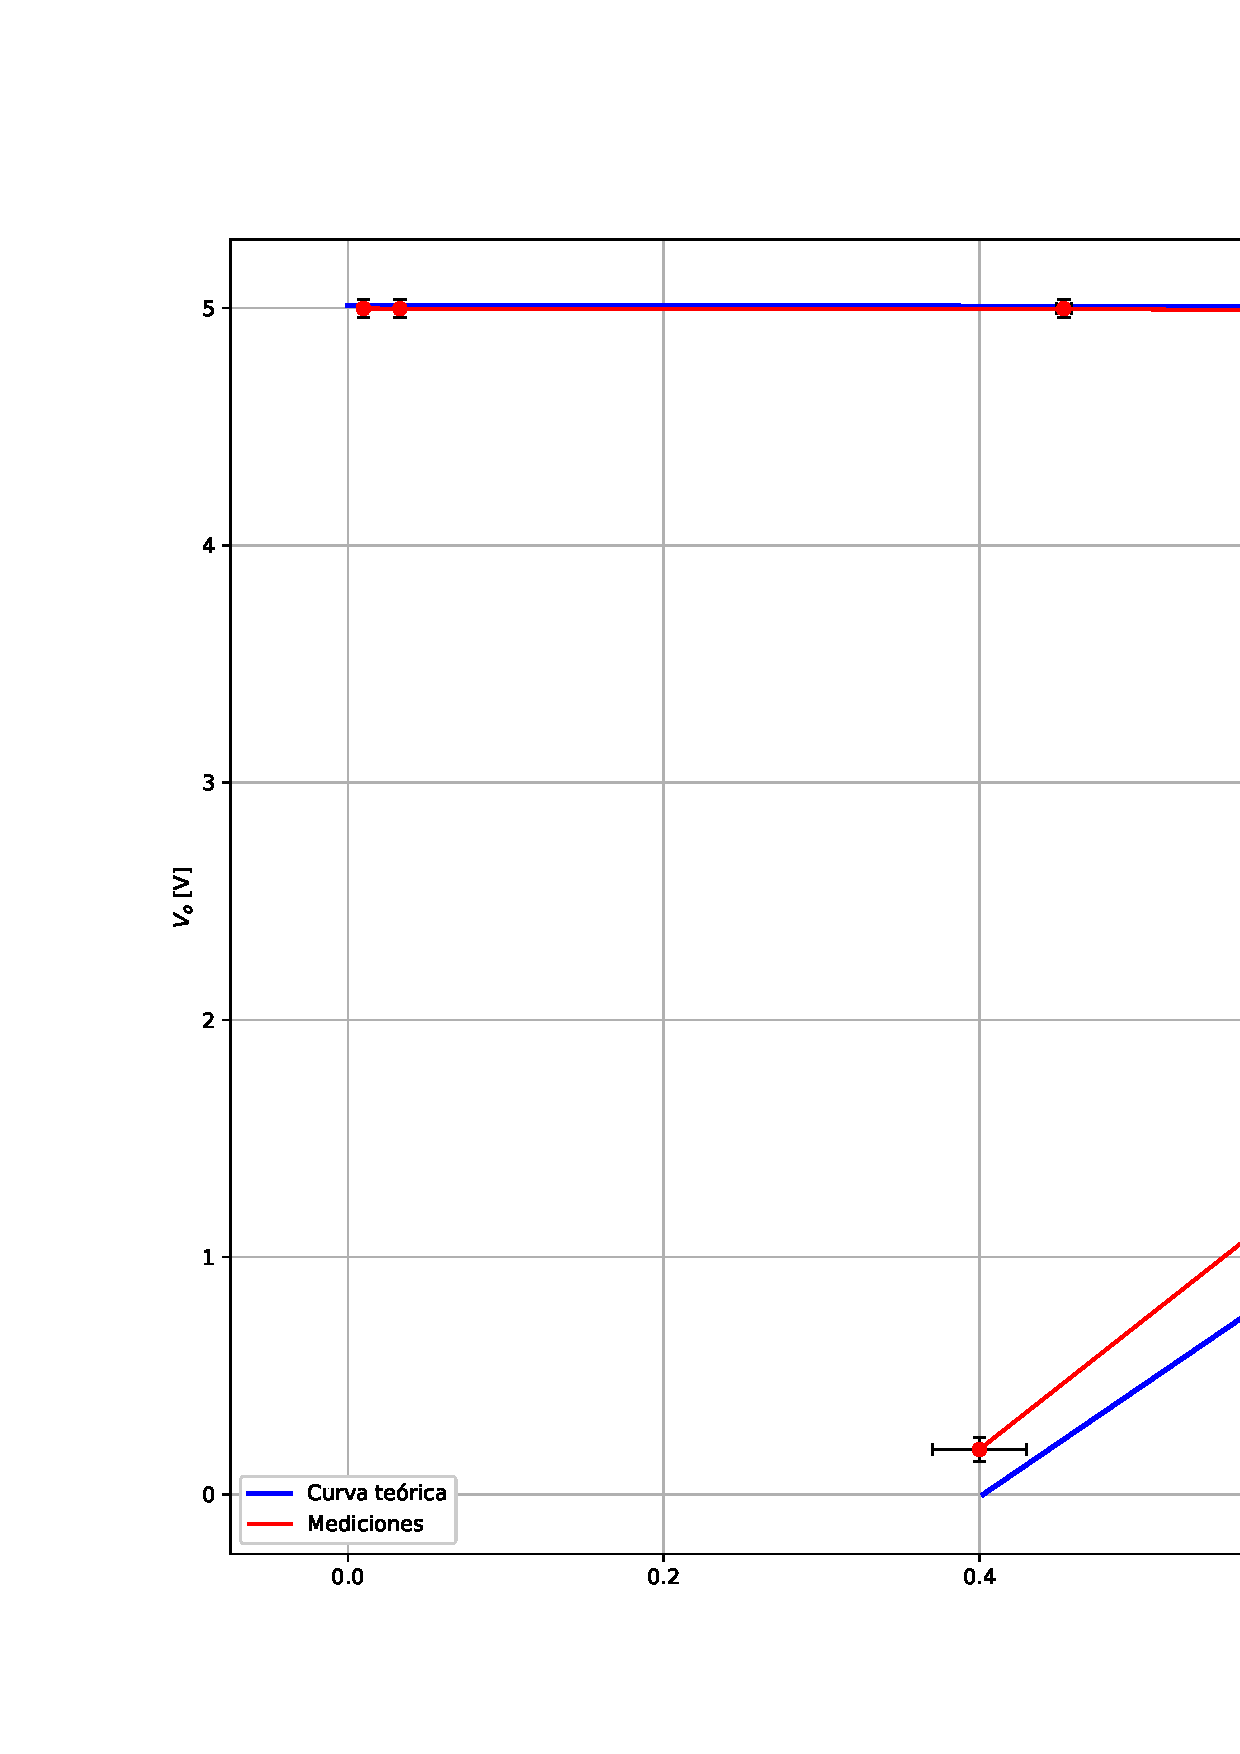
\includegraphics[width=\linewidth]{res/grafico_foldback.pdf} 
	\caption{Foldback medido superpuesto al simulado} 
	\label{fig:foldback} 
\end{figure}
%%%%%%%%%%%%%%%%%%%%%%%%%%%%%%%%%%%%%%%%%%%%%%%%%%%%%%%%%%%%%%%%%%%%
\subsection{Eficiencia}
\begin{figure}[H] 
	\centering 
	\includegraphics[width=\linewidth]{res/grafico_eficiencia_corriente.pdf} 
	\caption{Eficiencia contra corriente} 
	\label{fig:eficiencia_corriente} 
\end{figure}

\quad Primero se midió la eficiencia contra la corriente de salida, para esto se mantuvo la tensión de entrada en \SI{9.5}{V} y se hizo variar la carga entre los valores del rango de funcionamiento, midiendo las tensiones y corrientes tanto de entrada como de salida del circuito. 

\quad Como se puede ver en la curva de la \autoref{fig:eficiencia_corriente}, los valores rondan el 52\% de eficiencia, lo cual se corresponde con lo esperado. A bajas corrientes, la eficiencia cae porque la corriente de salida es del mismo orden que las corrientes internas de polarización, de modo que gran parte de la potencia de entrada no llega a la carga. Esto produce valores de eficiencia menores en el inicio de la curva.


\begin{figure}[H] 
	\centering 
	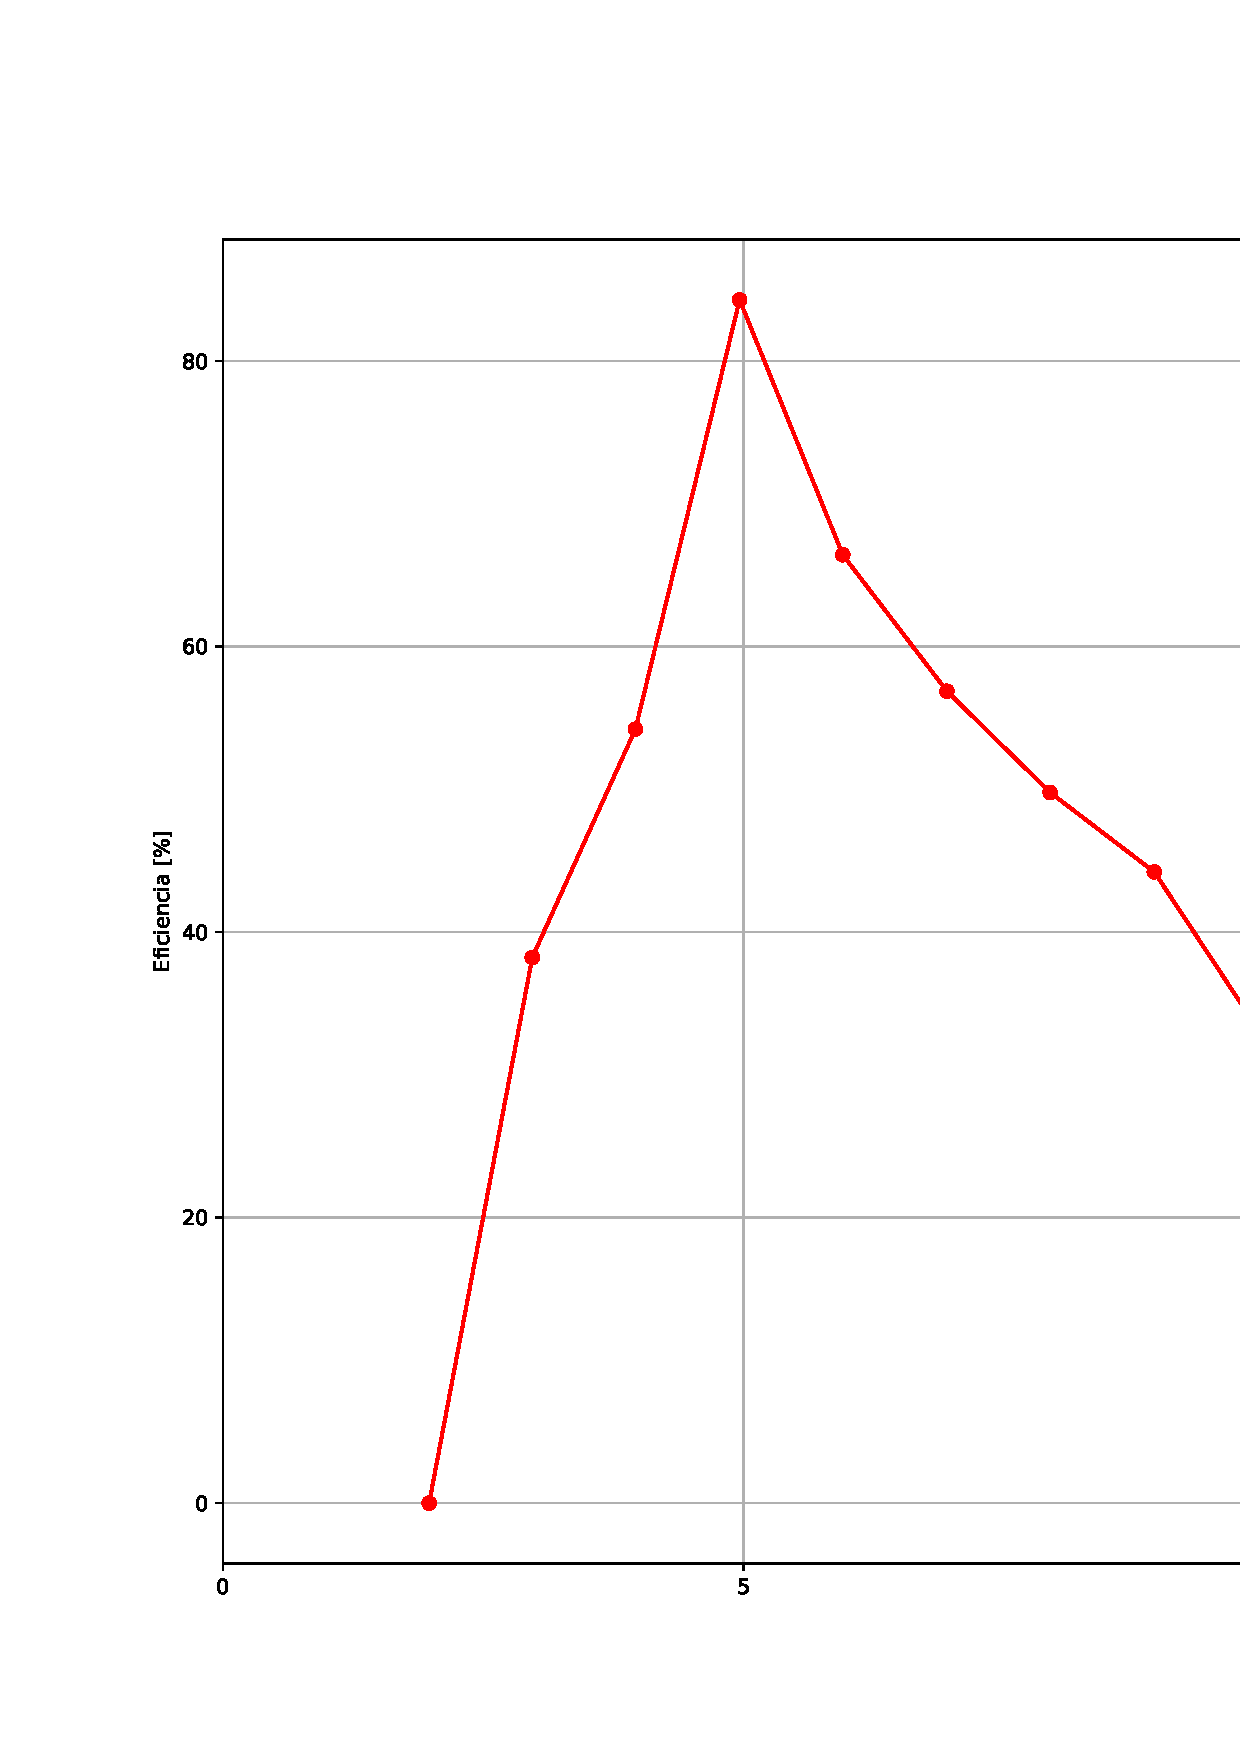
\includegraphics[width=\linewidth]{res/grafico_eficiencia_tension.pdf} 
	\caption{Eficiencia contra tensión} 
	\label{fig:eficiencia_tension} 
\end{figure}

\quad Luego se midió la eficiencia contra la tensión de entrada, para esto se mantuvo la carga constante en \SI{100}{\ohm} y nuevamente se midieron las tensiones y corrientes de entrada como de salida, variando la tensión de entrada entre \SI{0}{V} y \SI{24}{V}.

\quad Como se puede ver en la \autoref{fig:eficiencia_tension}, la eficiencia presenta un pico en \SI{5}{V} de entrada, aunque en este caso no es utilizable el circuito, ya que la tensión de salida no se encuentra dentro de las especificaciones. Luego, el decrecimiento a medida que aumenta la tensión de entrada es esperable, ya que aumenta la potencia de entrada mientras que la potencia de salida se mantiene constante. 


%%%%%%%%%%%%%%%%%%%%%%%%%%%%%%%%%%%%%%%%%%%%%%%%%%%%%%%%%%%%%%%%%%%%
\subsection{Tiempo de respuesta}
\quad Al momento de medir el tiempo de encendido y apagado del circuito se utilizó una resistencia en paralelo con un capacitor de 10$\Omega$ y 1$\mu$F respectivamente. Para medirlo se debió conectar y desconectar la fuente de alimentación. Con un osciloscopio se utilizaron ambos canales, uno para observar el tiempo de respuesta de la desconexión de la fuente y otro para observar el tiempo de respuesta del circuito. Se consiguieron los siguientes gráficos. 
\begin{figure}[H] 
	\centering 
	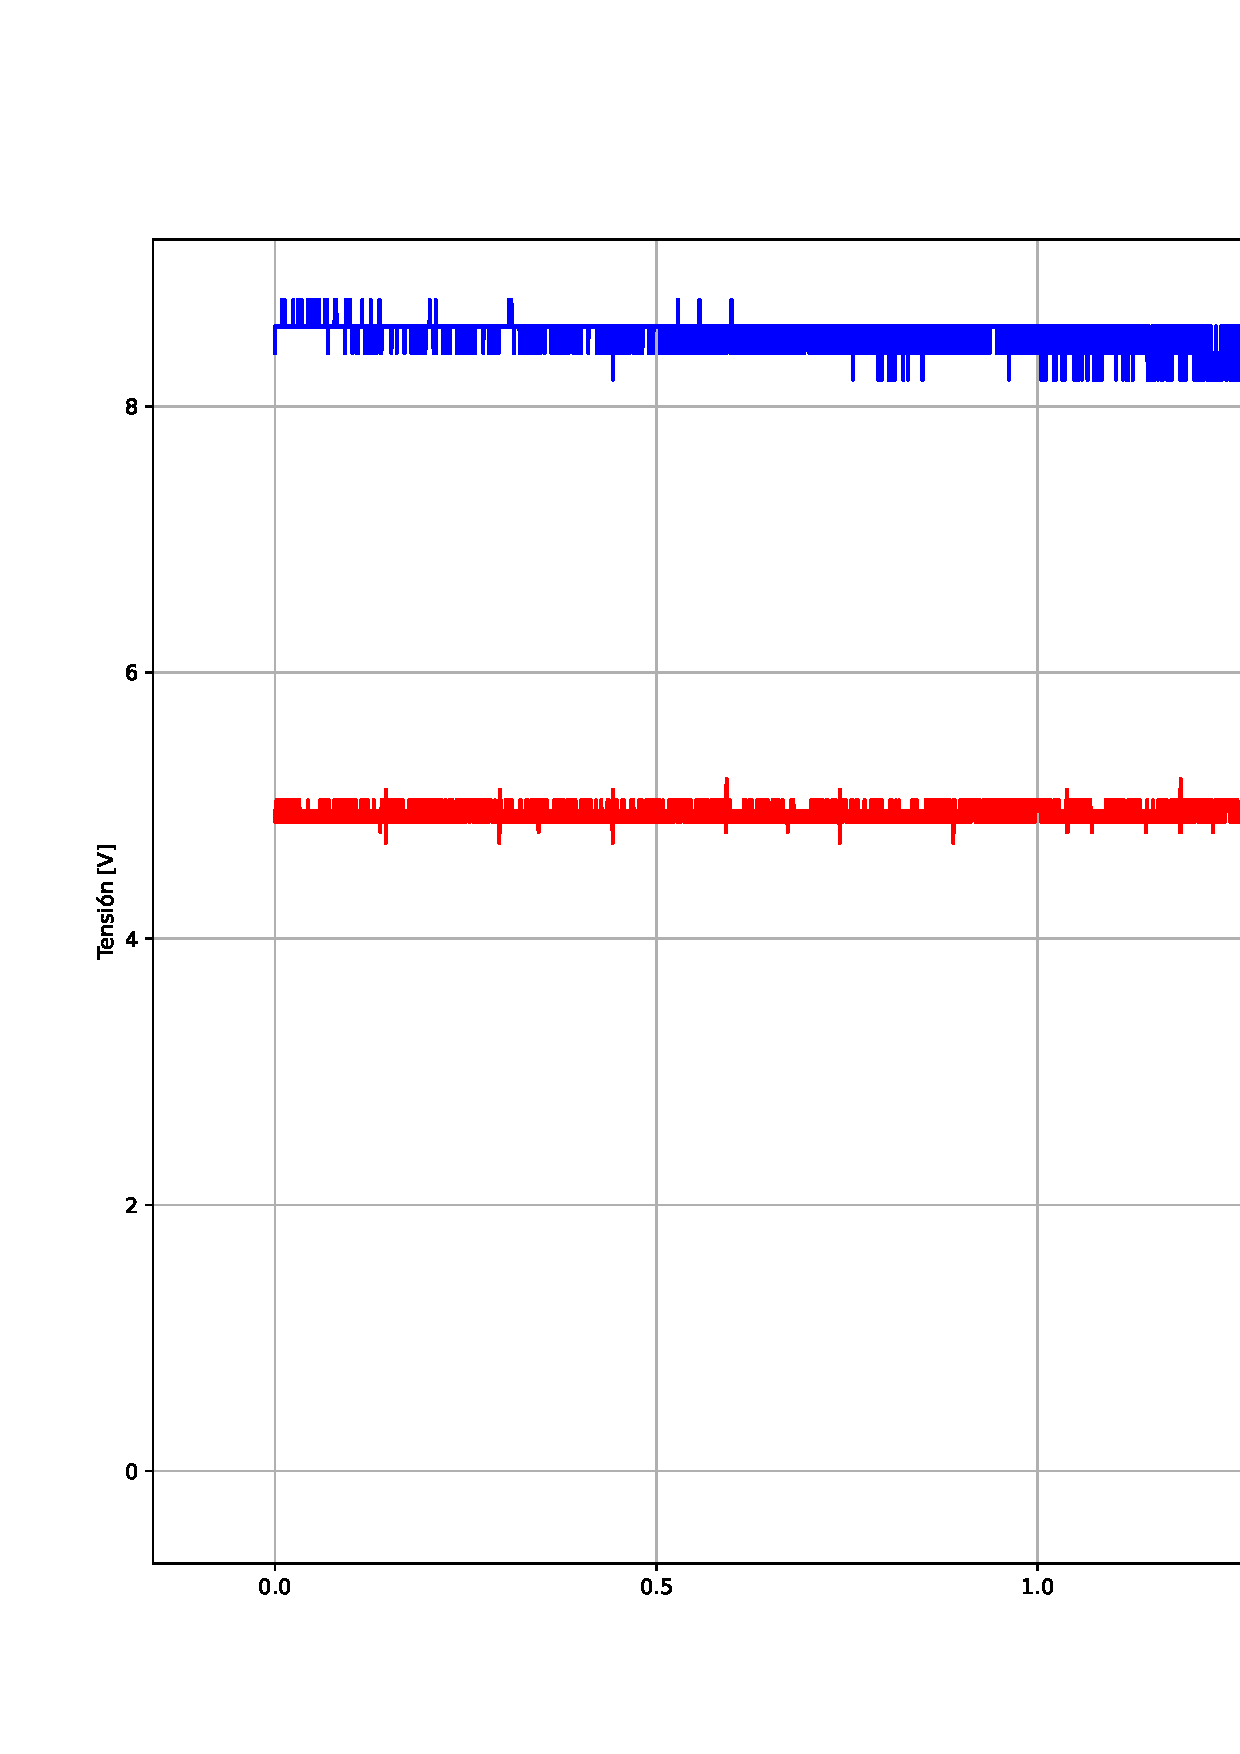
\includegraphics[width=\linewidth]{res/grafico_tiempo_apagado.pdf} 
	\caption{Tiempo de respuesta apagado} 
	\label{fig:tiempo_apagado} 
\end{figure}

\begin{figure}[H] 
	\centering 
	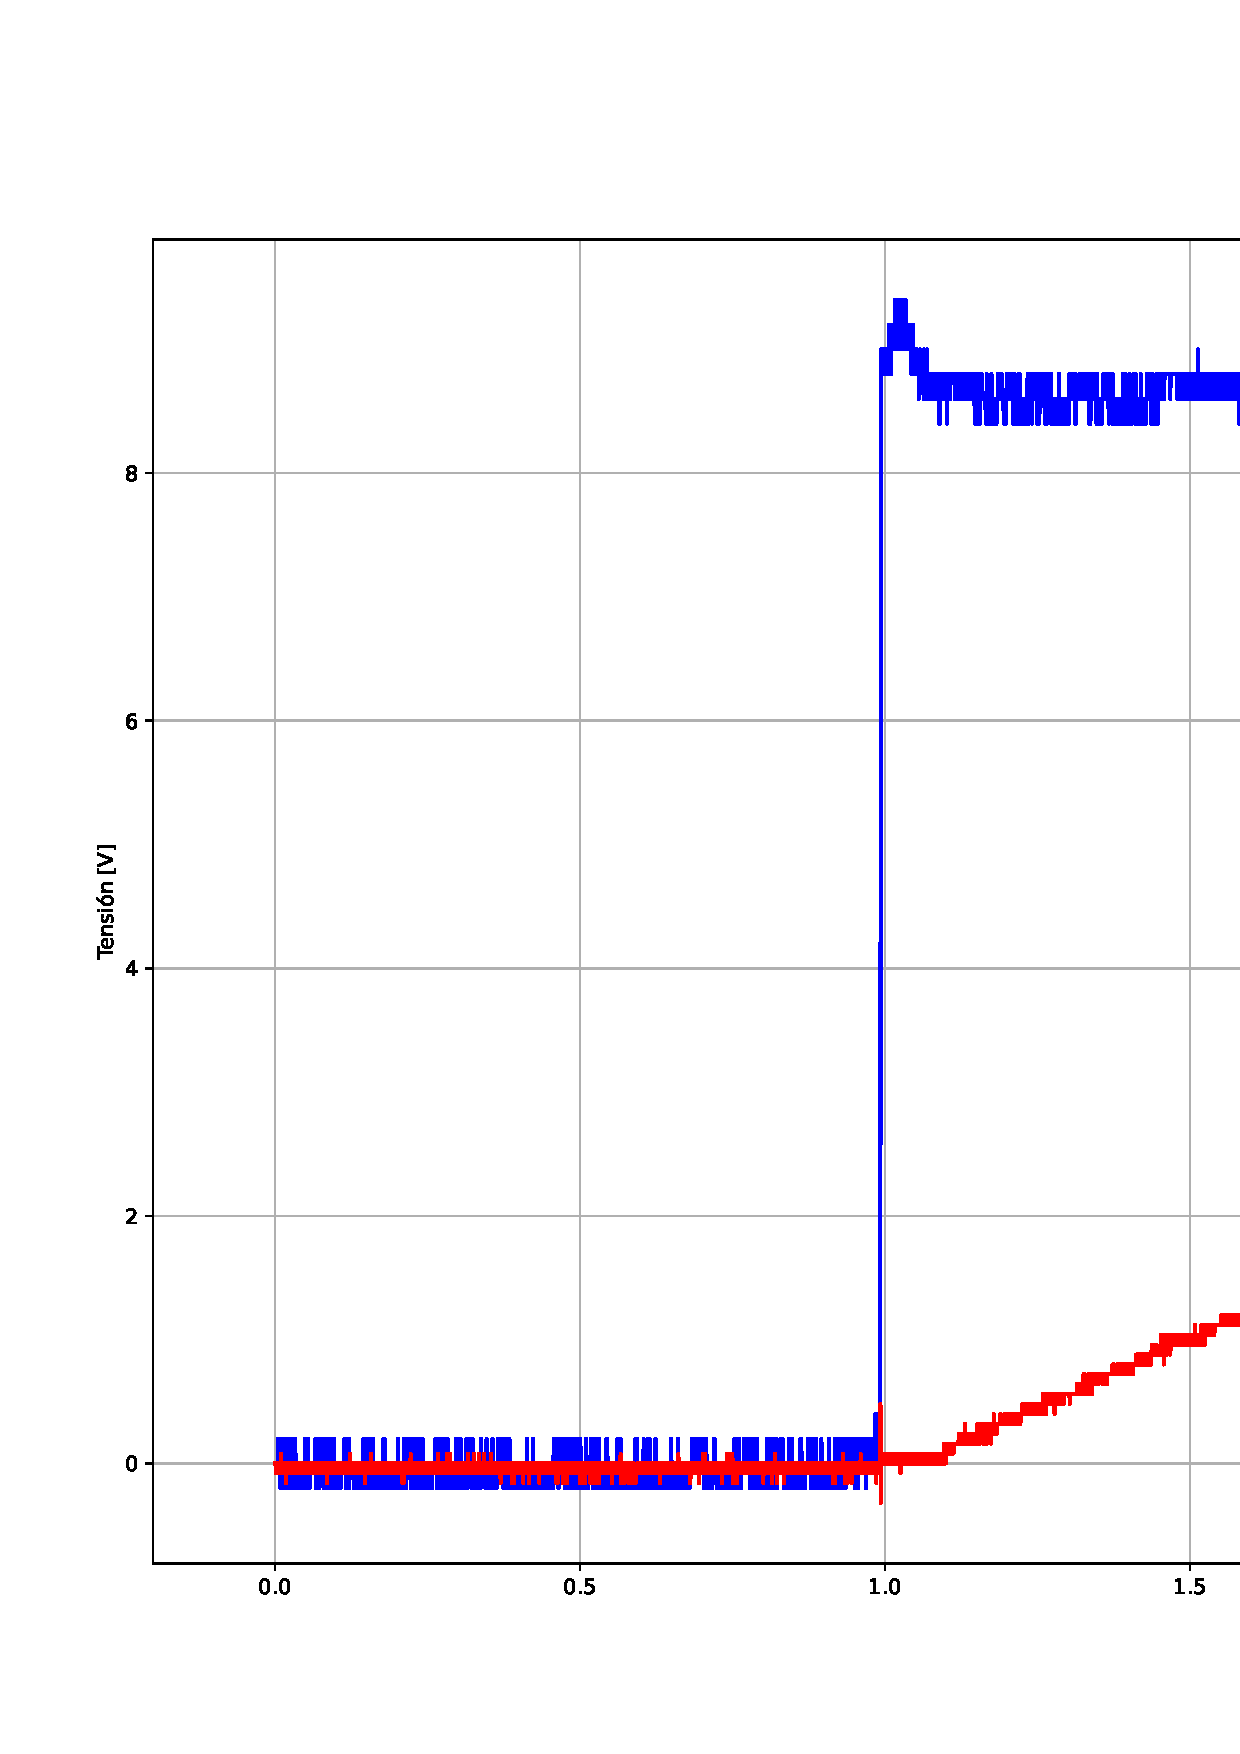
\includegraphics[width=\linewidth]{res/grafico_tiempo_encendido.pdf} 
	\caption{Tiempo de respuesta encendido} 
	\label{fig:tiempo_encendido} 
\end{figure}

En la \autoref{fig:tiempo_apagado} se observa un tiempo de apagado de \SI{0.4}{ms}. En la \autoref{fig:tiempo_encendido} se observa un tiempo de encendido de \SI{2.5}{ms}. 

\begin{figure}[H] 
	\centering \includegraphics[width=\linewidth]{res/grafico_carga_dinamica.pdf} 
	\caption{Regulación de carga dinámica} \label{fig:reg_de_carga_din} 
\end{figure}

\quad En la \autoref{fig:reg_de_carga_din} se puede ver la respuesta ante una carga dinámica, en este caso pasando de una corriente de salida de \SI{128}{\milli \ampere} a una corriente de salida de \SI{406}{\milli \ampere}. Se puede ver que la tensión cae aproximadamente \SI{200}{\milli \volt}, pero se restablece luego de aproximadamente \SI{14}{\milli \second}.

%%%%%%%%%%%%%%%%%%%%%%%%%%%%%%%%%%%%%%%%%%%%%%%%%%%%%%%%%%%%%%%%%%%%
\subsection{Resultados}

A continuación se muestran los principales resultados obtenidos:

\begin{table}[h!]
	\centering
	\begin{tabular}{|c|c|c|}
		\hline
		Característica & Simulado & Medido      \\ \hline
		Tiempo de encendido   & $-$      & $2.5ms$      \\ \hline
		Tiempo de apagado     & $-$      & $0.4ms$       \\ \hline
		Regulación de linea   & $2.86$   & $1.75$         \\ \hline
		Regulación de carga    & $2.72m \ohm$ & $23.5m \ohm$  \\ \hline
	\end{tabular}
	\caption{Resultados}
	\label{tab:resultados}
\end{table}


\subsection{Conclusiones}


\quad En este trabajo se pudo armar el circuito diseñado en las entregas anteriores, verificando su funcionamiento dentro de las especificaciones y simulaciones. Las mediciones resultaron coherentes con lo diseñado, y en algunos casos hasta mejores que lo simulado. 
%%%%%%%%%%%%%%%%%%%%%%%%%%%%%%%%%%%%%%%%%%%%%%%%%%%%%%%%%%%%%%%%%%%%
\subsection{Anexo}
\subsubsection{Propagación de errores}

\quad Al momento de analizar los errores en la medición se debió tener en cuenta la dispersión de los multímetros y resistencias utilizados. Los multímetros con los que se realizaron las mediciones son: "UT890C", "UT139". Observando las especificaciones del fabricante se aprecia lo siguiente:
\begin{table}[h!]
	\centering
	\begin{tabular}{|c|c|c|}
		\hline
		\textbf{Magnitud} & \textbf{Rango} & \textbf{Resolución / Precisión} \\ \hline
		
		\multirow{2}{*}{UT890C DC Current} 
		& 600 mA & (1.2\% + 5) \\ \cline{2-3}
		& 20 A & (2.0\% + 5) \\ \hline
		
		\multirow{2}{*}{UT890C DC Voltage} 
		& 600 mV & (0.5\% + 4) \\ \cline{2-3}
		& 6 V &  (0.5\% + 2) \\ \hline
		
		\multirow{1}{*}{UT139 DC Current} 
		& 10 A & (0.7\% + 2) \\ \hline
		
		\multirow{1}{*}{UT139 DC Voltage} 
		& 600 V & (0.5\% + 2) \\ \hline
		
	\end{tabular}
	\caption{Incertezas de los multímetros UT890C y UT139}
	\label{tab:incertezas-multimetros}
\end{table}

\quad Con esta tabla y suponiendo un error del 5\% en todas las resistencias ya es posible realizar el cálculo de propagación de errores para los diferentes casos.


\paragraph{Error foldback}
\quad El error en la medición de foldback se calculó propagando el error de ambos multímetros y las resistencias para los diferentes valores de corriente y tensión. Se utilizó el UT890C para medir la corriente y el UT139 para medir la tensión. Entonces, el error estará dado por:

\quad $\Delta$ T + $\Delta$ I + $\Delta$ R

\quad Al momento de medir el error, se tomó que "Alta corriente" tiene una resolución de 0.01A y "Baja corriente" tiene una resolución de 0.1mA. El UT139 es de resolución variable. Existen cuatro casos de errores:

\quad 1. Alta tensión, baja corriente: \[
V = \big[(0.5\% V_{out} + 2) + 5\%R_L\big ]V 
\hspace{0.5cm} 
\text{y} 
\hspace{0.5cm} 
I = \big[(1.2\%I_{out} + 5) + 5\%R_L\big]A
\]


\quad 2. Alta tensión, alta corriente:  \[
V = \big[(0.5\%V_{out} + 2D) + 5\%R_L\big]V
\hspace{0.5cm}
\text{y}
\hspace{0.5cm}
I = \big[(2.0\%I_{out} + 5D) + 5\%R_L\big]A
\]

\quad 3. Baja tensión, alta corriente:  \[
V = \big[(0.5\%V_{out} + 2D) + 5\%R_L\big]V
\hspace{0.5cm}
\text{y}
\hspace{0.5cm}
I = \big[(2.0\%I_{out} + 5D) + 5\%R_L\big]A
\]

\quad 4. Baja tensión, baja corriente:  \[
V = \big[(0.5\%V_{out} + 2D) + 5\%R_L\big]V 
\hspace{0.5cm} 
\text{y} 
\hspace{0.5cm} 
I = \big[(1.2\%I_{out} + 5D) + 5\%R_L\big]I
\]

\newpage

\section{Cuarto checkpoint}

\subsection{Introducción}

\quad En esta entrega se realizara el diseño de la fuente buck y el circuito PWM. Para la fuente buck se deben realizar los cálculos necesarios para obtener las características físicas del inductor que se utilizara para implementar dicho circuito.  

\quad Ambos circuitos se deben diseñar teniendo en cuenta las especificaciones requeridas por el trabajo. La eficiencia para la fuente buck y la frecuencia para el PWM.
%%%%%%%%%%%%%%%%%%%%%%%%%%%%%%%%%%%%%%%%%%%%%%%%%%%%%%%%%%%
\subsection{Fuente buck}
%%%%%%%%%%%%%%%%%%%%%%%%%%%%%%%%%%%%%%%%%%%%%%%%%%%%%%%%%%%
\subsubsection{Diseño y simulación}
\quad En las fuentes buck se busca reducir la tensión de entrada a un nivel inferior en la salida, manteniendo la alta eficiencia. Para ello se utilizan distintos componentes. Un MOSFET canal N (IRFZ44N) es utilizado para actuar como interruptor controlado por PWM (debido a este comportamiento de "llave", la tensión Drain-Source de este MOSFET es muy baja); el segundo NMOS (IRFZ44N) conduce la corriente cuando el primer transistor se encuentra apagado, implementando de esta manera las llaves ideales vistas en el circuito teórico. 

\quad También se agregan capacitores para evitar picos de tensión. El circuito cuenta además con un inductor, el cual almacena energía y suaviza la corriente. Este inductor debe calcularse con precisión para evitar sobrecalentamientos, tener tiempos de respuesta acordes y otros factores; es por esto que se le dedicará toda una sección a su diseño.

\quad Para obtener el valor de la inductancia primero se calculo el mínimo valor que puede tomar para que el circuito continúe funcionando de manera adecuada. Para eso se debió considerar el caso de mayor conmutación, en donde la resistencia de carga es máxima. 
\begin{equation*}
	R_{max} = \frac{V_o}{I_{s,min}} 
\end{equation*}
\quad Considerando que $V_o=9.5V$ y $I_{s,max} =$\SI{0.1}{\ampere} se obtiene $R_{max} = 95\ohm$. Luego, el inductor se calcula mediante la siguiente expresión.
\begin{equation}
	L_{cr} = \frac{(1-D)R_{max}}{2f}
\end{equation}
\quad Considerando que se va a tener un  $D_{min}$ y un $D_{max}$ dependiendo de la $V_{in}$ se calcularon ambos:
\begin{equation}
	D_{max} = \frac{V_o + V_{ds2}}{V_{in}-V_{ds1}+V_{ds2}} = \frac{9.5+0.049}{12} = 0.7957
\end{equation}
\begin{equation}
	D_{min} = \frac{V_o + V_{ds2}}{V_{in}-V_{ds1}+V_{ds2}} = \frac{9.5+0.049}{30} = 0.3183
\end{equation}
\quad Se calcularon dos valores de $L_{cr}$ y se utilizó el más alto de ambos que es el que cumple con lo pedido y presenta el peor caso para el inductor critico. 
\quad De las cuentas se obtuvo $L_{cr} =$\SI{250}{\micro\henry}. Sin embargo, se decidió utilizar un inductor L = \SI{300}{\micro\henry} para mayor seguridad y evitar que variaciones en el valor real del inductor presenten problemas graves en el circuito implementado.

\quad El valor del capacitor de salida se debe calcular considerando el ripple, por lo tanto el valor se calculo de manera iterativa. Se decidió un valor inicial de \SI{100}{\micro F} y se observo el valor del ripple con ese valor para luego poder aplicar la siguiente expresión:
\begin{equation}
	\Delta V_o = \frac{I_{L,max}-I_{L,min}}{8Cf}
\end{equation}
\quad Con un capacitor de \SI{47}{\micro F} se obtiene un $\Delta V_o = $\SI{2.5}{\milli V} que cumple con los requisitos de tension de salida.

\quad Una vez finalizado todo el desarrollo del circuito se consiguió el siguiente diseño.

\begin{figure}[H]
	\centering
	\includegraphics[width=\linewidth]{res/simulacion_buck.png}
	\caption{Circuito Fuente Buck}
	\label{fig:simulacion_buck}
\end{figure}

\quad La tensión de salida de la fuente buck:

\begin{figure}[H]
	\centering
	\includegraphics[width=\linewidth]{res/simu_vo_buck.png}
	\caption{Tension de salida de la fuente buck}
	\label{fig:vo_buck}
\end{figure}

\quad La corriente sobre el inductor:
\begin{figure}[H]
	\centering
	\includegraphics[width=\linewidth]{res/simu_il_buck.png}
	\caption{Corriente sobre el inductor}
	\label{fig:corriente_inductor}
\end{figure}

\quad En la \autoref{fig:vo_buck} se puede ver que, además de la oscilación, el valor medio no es constante, esto se atribuye a la necesidad de agrandar el error de convergencia admitido para asegurarse esta misma.
%%%%%%%%%%%%%%%%%%%%%%%%%%%%%%%%%%%%%%%%%%%%%%%%%%%%%%%%%%%
\subsubsection{Inductor}

\quad Al momento de diseñar el inductor se debieron tener en cuenta ciertos parámetros de funcionamiento de la fuente buck. La frecuencia trabajo es de \SI{130}{kHz}, la $I_{L_{max}} = 1.54 A $, la $I_{L_{min}} = 1.42 A$.

\quad Se obtuvieron las características físicas del inductor usando el método \textit{Tacca}. Se debe considerar $\sigma_{IL} \leq 5 \frac{A}{mm^2}$ para evitar el sobrecalentamiento del alambre. Considerando los núcleos disponibles comercialmente y la tabla de cables provista por \textit{Ericksson}, se realizaron los cálculos necesarios para obtener los siguientes parámetros.

\begin{table}[H]
	\centering
	\begin{tabular}{|c|c|}
		\hline
		\textbf{Parámetros} & \textbf{Valor} \\ \hline
		Material del nucleo  & \textit{N87} \\ \hline
		Nucleo &  EE3007\\ \hline
		Cable de cobre &  AWG\#20\\ \hline
		Inductancia [$\mu$ Hy] & 300 \\ \hline
		$l_g$ [mm]& 0.151 \\ \hline
		Numero de vueltas & 25 \\ \hline
		$\sigma_{IL} [\frac{A}{mm^2}]$ & 2.978 \\ \hline
		$r_{Cu}$ [cm] & 0.0437 \\ \hline
		$\delta$ [cm] & 0.021 \\ \hline
	\end{tabular}
	\caption{Especificaciones del inductor}
	\label{tab:especif_inductor}
\end{table}
\quad Con los valores obtenidos no hay efecto pelicular. 

%%%%%%%%%%%%%%%%%%%%%%%%%%%%%%%%%%%%%%%%%%%%%%%%%%%%%%%%%%%
\subsubsection{Eficiencia}
\quad En los reguladores conmutados Buck una eficiencia ideal sería del $100\%$. Sin embargo, esta eficiencia resulta imposible en la realidad debido a perdidas por conmutación, resistencias parasitas, caídas en el MOSFET, entre otros factores. Debido a esto, la eficiencia real estará alrededor del $90\% - 95\%$. Esta eficiencia aumentará dependiendo de la optimización del PCB, un control preciso del ciclo de trabajo y un MOSFET acorde. 

\quad En el caso del circuito diseñado, al utilizar un MOSFET como reemplazo del diodo para la conmutación, se logra una reducción en la caída de tensión. Además, la elección del inductor y el capacitor logran una gran reducción en el ripple de corriente y tensión respectivamente, lo que mejora la eficiencia.

\quad La eficiencia del circuito se obtiene segun la siguiente expresión:
\begin{equation}
	eficiencia  = \frac{P_{salida}}{P_{entrada}}
\end{equation}
\begin{equation}
	\eta (9.3V)  = \frac{9.3*1.469}{24*0.00631} = 90.2\%
\end{equation}
\begin{equation}
	\eta(9.7V) = \frac{9.7*0.103}{24*0.045} = 91.5\%
\end{equation}
\quad Ambos resultados cumplen con la eficiencia pedida para ambas tensiones especificadas del regulador buck.
%%%%%%%%%%%%%%%%%%%%%%%%%%%%%%%%%%%%%%%%%%%%%%%%%%%%%%%%%%%
\subsubsection{Diseño de PCB}
\quad Para realizar el PCB de la fuente buck debió tenerse en cuenta el trazado de pistas. Aquí se tuvo en cuenta la separación entre ellas para así evitar capacitancias o inductancias parásitas. Además se debió mantener un cierto ancho de las pistas debido a la potencia que circula en ciertas zonas. Se planeó previamente el plano de masa para así mejorar el retorno de la corriente y reducir ruido. Teniendo todas estas cuestiones en consideración se obtuvo el siguiente diseño.

\begin{figure}[H]
	\centering
	\includegraphics[width=\linewidth]{res/pcb_buck.jpg}
	\caption{Diseño PCB frente Fuente Buck}
	\label{fig:pcb_frente_buck}
\end{figure}
\begin{figure}[H]
	\centering
	\includegraphics[width=\linewidth]{res/pcb_buck_dorso.jpg}
	\caption{Diseño PCB dorso Fuente Buck}
	\label{fig:pcb_dorso_buck}
\end{figure}
%%%%%%%%%%%%%%%%%%%%%%%%%%%%%%%%%%%%%%%%%%%%%%%%%%%%%%%%%%%
\subsection{Circuito PWM}

\quad Como se mencionó antes, para la fuente buck se necesita una señal PWM que se ocupará de encender y apagar los MOSFETs. La forma de obtener tal señal utilizada es mediante la comparación de una señal triangular de \SI{130}{\kilo hz} con una tensión constante. La ventaja de obtener la señal PWM de esta forma es que la tensión constante que se compara con la señal triangular podrá ser una señal proporcional a el error de la tensión de salida con la tensión deseada, de esta forma cerrando el lazo y obteniendo una fuente buck a lazo cerrado.

%%%%%%%%%%%%%%%%%%%%%%%%%%%%%%%%%%%%%%%%%%%%%%%%%%%%%%%%%%%
\subsubsection{Diseño y simulación}

\quad La topología utilizada para obtener la señal deseada es la de la \autoref{fig:esquema_pwm}. Este circuito consta de un integrador con el operacional U2 y el capacitor, que recibe una señal cuadrada de la salida de U1, generando la triangular deseada, que luego se compara con V3 en U3, para finalmente tener la señal PWM deseada. Dado la alta frecuencia de oscilación utilizada, U1 y U3 son comparadores en vez de amplificadores operacionales.

\begin{figure}[H]
	\centering
	\includegraphics[width=\linewidth]{res/esquema_pwm.png}
	\caption{Circuito utilizado para generar la señal PWM}
	\label{fig:esquema_pwm}
\end{figure}

\quad Los valores utilizados para los resistores y capacitores son los presentados en la \autoref{tab:valores_comp_pwm}. Los mismos se obtuvieron de forma empírica, teniendo en cuenta la constante de tiempo $\tau = R3 \cdot C$.

\begin{table}[H]
	\centering
	\begin{tabular}{|c|c|}
		\hline
		\textbf{Componente} & \textbf{Valor} \\ \hline
		R1 & \SI{100}{\kilo \ohm} \\ \hline
		R2 & \SI{24}{\kilo \ohm} \\ \hline
		R3 & \SI{2.7}{\kilo \ohm} \\ \hline
		C & \SI{2.2}{nF} \\ \hline
	\end{tabular}
	\caption{Valores de los componentes del circuito PWM}
	\label{tab:valores_comp_pwm}
\end{table}
\quad Al simular el circuito se obtuvieron las señales cuadrada y triangular de las figuras \ref{fig:simu_pwm_cuad} y \ref{fig:simu_pwm_triang}: 

\begin{figure}[H]
	\centering
	\includegraphics[width=\linewidth]{res/grafico_simu_pwm_cuad.png}
	\caption{Señal cuadrada simulada}
	\label{fig:simu_pwm_cuad}
\end{figure}

\begin{figure}[H]
	\centering
	\includegraphics[width=\linewidth]{res/grafico_simu_pwm_triang.png}
	\caption{Señal triangular simulada}
	\label{fig:simu_pwm_triang}
\end{figure}
%%%%%%%%%%%%%%%%%%%%%%%%%%%%%%%%%%%%%%%%%%%%%%%%%%%%%%%%%%%
\subsubsection{Diseño de PCB}

\begin{figure}[H]
	\centering
	\includegraphics[width=0.5\linewidth]{res/pcb_pwm.png}
	\caption{Circuito PCB PWM}
	\label{fig:pcb_pwm}
\end{figure}
\begin{figure}[H]
	\centering
	\includegraphics[width=0.5\linewidth]{res/pcb_pwm_frente.png}
	\caption{Circuito PCB PWM}
	\label{fig:pcb_pwm_frente}
\end{figure}
\quad Al momento de realizar el diseño del PCB se debieron tener en cuenta las consideraciones nombradas anteriormente. Ademas se tuvo presente que las pistas debían evitar recorridos de gran distancia ya que al transportar frecuencia si estas son muy largas se puede generar ruido en la información. 

\quad Se agregaron pines de prueba al circuito en lugares estratégicos para luego poder verificar el funcionamiento del circuito, pudiendo observar la señal en donde es necesario que cumplan con formas y frecuencias especificas. Por lo tanto los pines agregados son en tierra, en la salida del comparador y en la salida del integrador. 

\quad Ademas como los comparadores son \textit{open collector} se agregaron resistencias de pull up conectadas a su salida. Se eligió el valor teniendo en cuenta lo recomendado por la datasheet del modelo y buscando evitar que se limite la corriente. 

\begin{figure}[H]
	\centering
	\includegraphics[width=0.5\linewidth]{res/pwm_frente.jpeg}
	\caption{Circuito PWM}
	\label{fig:pwm_frente}
\end{figure}

\begin{figure}[H]
	\centering
	\includegraphics[width=0.5\linewidth]{res/pwm_atras.jpeg}
	\caption{Circuito PWM}
	\label{fig:pwm_dorso}
\end{figure}

\quad Durante la implementación se observo que el valor de capacitancia elegido inicialmente era muy cercano al del capacitor interno del operacional y por lo tanto se deformaba la señal. Para solucionarlo se cambio la relación del RC, se aumento el valor del capacitor y se disminuyo el de la resistencia.
%%%%%%%%%%%%%%%%%%%%%%%%%%%%%%%%%%%%%%%%%%%%%%%%%%%%%%%%%%
\subsubsection{Mediciones}
\quad Al llevar a cabo las mediciones, se observó la señal cuadrada generada por el circuito a una frecuencia aproximada de 130kHz, tal como fue diseñada. Esta señal presenta transiciones rápidas por lo que se garantiza una conmutación correcta y eficiente de los MOSFETs en la fuente Buck. La amplitud de la señal se mantiene estable en el tiempo, sin ningún tipo de distorsiones.

\quad Por otro lado, la señal triangular muestra una forma simétrica y estable con una amplitud adecuada. Se observó que la frecuencia de oscilación también es de aproximadamente 130KHz.

\quad Se puede observar una distorsión en la señal triangular que se genera debido a la integración del sobrepico en la señal cuadrada. 

\quad Las posibles causas de este sobrepico son el problema ya antes mencionado de las capacidades de entrada del operacional o interferencias causadas por ruido generado en las pistas del PCB. 

\quad A pesar de lo mencionado, estas mediciones se puede confirmar el correcto funcionamiento del PWM, asegurando así una señal de control para la fuente conmutada Buck estable cumpliendo todos los requisitos.
\begin{figure}[H]
	\centering
	\includegraphics[width=\linewidth]{res/cuadrada.pdf}
	\caption{Señal cuadrada}
	\label{fig:seña_cuadrada}
\end{figure}
\begin{figure}[H]
	\centering
	\includegraphics[width=\linewidth]{res/senal_triangular.pdf}
	\caption{Señal triangular}
	\label{fig:señal_triangular}
\end{figure}
%%%%%%%%%%%%%%%%%%%%%%%%%%%%%%%%%%%%%%%%%%%%%%%%%%%%%%%%%%%
\subsection{Conclusiones}
\quad A lo largo del desarrollo se abordó el diseño y simulación de una fuente conmutada tipo Buck, donde se debió trabajar el control por modulación de ancho de pulso y el diseño físico del inductor. Durante la simulación, se observo que esta fuente Buck cumplió los requerimientos, superando el 90\% de eficiencia en distintas condiciones de carga, manteniendo a su vez un tiempo de establecimiento y un ripple acorde. 

\quad Se puso en práctica el diseño de pistas para circuitos de frecuencia, en donde se tuvo que considerar el trazado de pistas y el plano de masa. 
El diseño del circuito PWM se implementó mediante comparadores, logrando generar, luego de varios intentos, una señal triangular estable y una señal PWM capaz de controlar los MOSFETs.
%%%%%%%%%%%%%%%%%%%%%%%%%%%%%%%%%%%%%%%%%%%%%%%%%%%%%%%%%%%
\subsection{Apéndice}
%%%%%%%%%%%%%%%%%%%%%%%%%%%%%%%%%%%%%%%%%%%%%%%%%%%%%%%%%%%
\subsubsection{Calculo del inductor}

\quad Se utilizaron las siguientes especificaciones para realizar los cálculos:
\begin{center}
	\begin{equation*}
		\begin{aligned}
			L &= \SI{300}{\micro\henry} \\
			I_{L,max} &= \SI{1.54}{\ampere} \\
			I_{L,dc} &= \SI{1.48}{\ampere} \\
			f_{sw} &= \SI{130}{\kilo\hertz} \\
			P_{cu} &= \SI{1}{\watt} \\
			K_u &= 0{,}33 \\
			\rho_{cu} &= \SI{1.7e-6}{\ohm\centi\metre}
		\end{aligned}
	\end{equation*}
\end{center}
\quad El campo magnético máximo se obtuvo de la hoja de datos del material observando el máximo valor donde la permeabilidad tiene un comportamiento lineal.Luego, los valores de corriente máxima y media fueron obtenidos cuando la carga es mínima $R_{L_{min}} = \frac{9V}{1.5A} = 6.33\ohm$

\quad El método \textit{Tacca} indica que en primer lugar se debe calcular la sección de hierro, $S_{fe}$.
\begin{center}
	\begin{equation*}
		\begin{aligned}
			F_b &= K_u \\
			F_v &= 0.25 \\
			I_{L,ef} &= I_{L,dc} \\
			\sigma_{IL} &= \SI{5}{ \frac{\ampere}{\milli\metre^2}}
		\end{aligned}
	\end{equation*}
\end{center}

\begin{equation}
	S_{fe} = 10\sqrt{\frac{LI_{L,ef}I_{L,max}}{F_bF_vB_{max}\sigma_{IL}}} = 0.744 cm^2 
\end{equation}
\quad Verificando la tabla provista por \textit{Ericksson} y la disponiblidad comercial, se decidio usar el nucleo \textit{EE3007}. Una vez decidido el nucleo es necesario verificar el valor del facotr de ventana, $F_v$, elegido. Para eso se utilizo la datasheet del nucleo para obtener las dimensiones de la pieza.
\begin{center}
	\begin{equation*}
		\begin{aligned}
			B &= \SI{19,6}{\milli\metre} \\
			C &= \SI{9,5}{\milli\metre} \\
			D &= \SI{6,5}{\milli\metre} \\
			E &= \SI{6,3}{\milli\metre} \\
			F &= \SI{6,3}{\milli\metre} \\
		\end{aligned}
	\end{equation*}
\end{center}
\begin{equation}
	F_v = \frac{S_v}{S_{fe}} = \frac{E(B-C)}{2CD} = 0.35
\end{equation}
\quad Considerando este valor se volvió a calcular la sección del hierro, $S_{fe} =\SI{0.629}{\centi\metre^2}$. La variación es pequeña por lo que la elección del nucleo continua cumpliendo. 

\quad Se procedió a calcular el valor del entrehierro. 
\begin{equation}
	12 \frac{L}{S_{fe}}(\frac{I_{L,max}}{B_{max}})^2 =\SI{0.151}{\milli\metre} 
\end{equation}

\quad Obtenido este valor, se pudo conseguir el numero de vueltas necesarias para el inductor. 
\begin{equation}
	n = 850\frac{B_{max}}{I_{L,max}}I_g = 25
\end{equation}

\begin{center}
	\begin{equation*}
		\begin{aligned}
			W_a = \SI{0.476}{\centi\metre^2}
		\end{aligned}
	\end{equation*}
\end{center}
\begin{equation}
	A_w \leq\frac{K_uW_a}{n} = \SI{6.283e-3}{\centi\metre^2}
\end{equation}
\quad Se elige usar el camble AWG\#20 que tiene un $A_w = \SI{5.188e-3}{\centi\metre^2}$. Se verifica que el valor de la densidad sea menor a \SI{5}{\frac{\ampere}{\milli\metre^2}} y que no sature
\begin{center}
	\begin{equation*}
		\begin{aligned}
			\sigma_{IL} = \frac{I_{L,max}}{100A_w} = \SI{2.789}{\frac{\ampere}{\milli\metre^2}} \\
			B_{max,real} = \frac{\mu_0nI_{L,max}}{I_g} = \SI{0.0003}{T}
		\end{aligned}
	\end{equation*}
\end{center}

\quad Finalmente, se verifico que no haya efecto pelicular, es decir que $\delta\leq r_{Cu}$. 
\begin{center}
	\begin{equation*}
		\begin{aligned}
			r_{Cu} =\SI{0.0437}{\centi\metre}\\
			\delta = \frac{7.5}{\sqrt{f_{sw}}} = 0.021
		\end{aligned}
	\end{equation*}
\end{center}

\newpage

\section{Quinto checkpoint}

\subsection{Introducción}
 

\quad En este trabajo se continuara con el diseño de la fuente buck desarrollado en la entrega anterior. Se cerrara el lazo de la misma, generado una compensación que permitirá mejorar el margen de fase y conseguir una respuesta no oscilatoria. 

\quad Además se armara el inductor diseñado previamente, teniendo en cuenta las consideraciones necesarias para poder cumplir con los valores calculados. 

\quad Se buscara medir y comprobar el correcto funcionamiento de todo lo diseñado a lo largo del trabajo. Comprobando que la integración de todo el sistema funcione de la manera esperada, cumpliendo con los requisitos pedidos. 

%%%%%%%%%%%%%%%%%%%%%%%%%%%%%%%%%%%%%%%%%%%%%%%%%%%%%%%%%%%%%%%
\subsection{Fuente Buck realimentada}

\quad Para realimentar la fuente se utilizó la topología de la \autoref{fig:circuito_lazo_cerrado}, donde se sensa la tensión de salida con las resistencias $R18$ y $R19$, luego se utiliza el $U7$ como amplificador de error, utilizando una referencia de \SI{4.75}{V}. Por ultimo, esta señal de error se compara con una señal triangular, generada con el circuito de la entrega anterior con pequeñas modificaciones para que la amplitud sea de aproximadamente \SI{1.9}{V}. Luego de este comparador se obtiene una señal PWM que, a través del \textit{MOSFET Driver}, se utilizará para conmutar los transistores. De esta forma el ciclo de trabajo resulta proporcional a la tensión de salida, permitiendo así la regulación de linea y de carga. 

\begin{figure}[H]
    \centering
    \includegraphics[width=\linewidth]{res/circuito_lazo_cerrado.png}
    \caption{Lazo de realimentación de la fuente buck}
    \label{fig:circuito_lazo_cerrado}
\end{figure}

\quad Al simular el circuito realimentado en LTspice se obtuvo la respuesta de la \autoref{fig:respuesta_sin_compensar}. Es evidente que el circuito oscila, por lo que se debe agregar una red de compensación. La próxima sección se ocupará de esto. 

\begin{figure}[H]
    \centering
    \includegraphics[width=\linewidth]{res/grafico_respuesta_sin_compensar.pdf}
    \caption{Respuesta del circuito realimentado}
    \label{fig:respuesta_sin_compensar}
\end{figure}
%%%%%%%%%%%%%%%%%%%%%%%%%%%%%%%%%%%%%%%%%%%%%%%%%%%%%%%%%%%%%%%%%%%%%%%%%%%%%%
\subsection{Compensación}

\quad Se decidió utilizar una compensación de amplificación de error tipo III, es decir se compensó con un PID. En este tipo de compensación se obtiene un polo en el origen, dos ceros y dos polos a una mayor frecuencia. Los ceros sirven para compensar los polos complejos conjugados correspondientes a la respuesta de la fuente buck. De esta manera se obtuvo un mayor margen de fase a lazo cerrado, además de un mayor ancho de banda. 

\begin{figure}[H]
    \centering
    \includegraphics[width=0.5\linewidth]{res/red_compensacion.pdf}
    \caption{Red de compensación}
    \label{fig:circuito_compensacion}
\end{figure}

\quad La resistencia $R_{comp}$ y el capacitor $C_{comp}$ añaden un cero a la respuesta, y la $R_{FBT}$ y el $C_{ff}$ añaden otro. Estos ceros contrarrestan el efecto de los polos complejos conjugados provenientes de la buck como se menciono previamente. 

\quad Los otros dos polos están dados por $R_{ff}$ y $C_{ff}$, y por $R_{comp}$ y $C_{HF}$. Estos tienen una frecuencia mayor a la de los de la fuente buck. 

\quad Los valores obtenidos luego de normalizar fueron los siguientes: 

\begin{table}[H]
\centering
\begin{tabular}{|c|c|}
\hline
\textbf{Componente} & \textbf{Valor} \\ \hline
$R_{comp}$ & \SI{8.2}{\nano\farad}\\ \hline
$C_{comp}$ &  \SI{15}{\kilo\ohm}\\ \hline
$C_{FF}$ &  \SI{12}{\nano \farad}\\ \hline
$R_{FF}$ & \SI{2}{\kilo \ohm} \\ \hline
$C_{HF}$& \SI{180}{\pico\farad} \\ \hline
$R_{FBT}$& \SI{10}{\kilo\ohm}\\ \hline
$R_{FBB}$ & \SI{10}{\kilo\ohm} \\ \hline
\end{tabular}
\caption{Componentes para la compensación}
\label{tab:comp_pa_comp}
\end{table}

\quad Para simular el bode se modificó uno de los modelos promediados provisto en el campus. Este modelo reemplaza el comportamiento de computación lineal por una representación continua basada en el ciclo de trabajo promedio. Por lo tanto, se logra obtener un modelo linealizado del sistema

\begin{figure}[H]
    \centering
    \includegraphics[width=0.8\linewidth]{res/esquematico_modelo_promedio.png}
    \caption{Modelo promediado de la fuente buck compensada}
    \label{fig:esq_modelo_promediado}
\end{figure}

\quad Los bodes resultantes fueron los vistos a continuación:

\begin{figure}[H]
    \centering
    \includegraphics[width=\linewidth]{res/bode_sin_comp.pdf}
    \caption{Bode del circuito sin compensar}
    \label{fig:bode_sin_compensar}
\end{figure}

\begin{figure}[H]
    \centering
    \includegraphics[width=\linewidth]{res/bode_comp.pdf}
    \caption{Respuesta del circuito compensado}
    \label{fig:respuesta_compensada}
\end{figure}

\quad Como se ve en la \autoref{fig:respuesta_compensada} con la compensación se logró obtener un margen de fase de 80\degree. Este esta dado por la red de adelanto implementada con los ceros en las frecuencias de los polos complejos. Además la ganancia en altas frecuencias se ve atenuada de manera significativa gracias los polos de alta frecuencia, de esta manera se logra limitar el ruido de conmutación.

\quad Gracias a la compensación el sistema presenta una mayor estabilidad y robustez. La respuesta en frecuencia del circuito compensado presenta mejores características que la del mismo sin compensar. 

\begin{figure}[H]
    \centering
    \includegraphics[width=\linewidth]{res/grafico_respuesta_compensada.pdf}
    \caption{Respuesta del circuito realimentado compensado}
    \label{fig:grafico_respuesta_compensada}
\end{figure}
%%%%%%%%%%%%%%%%%%%%%%%%%%%%%%%%%%%%%%%%%%%%%%%%%%%%%%%%%%%%%%%%%%%%%%%%%%%%%%
\subsection{Caracterización del inductor}

\quad A la hora de corroborar el valor de la inductancia se utilizó un circuito RL, sabiendo que la relación entre la tensión de entrada y la tensión sobre el inductor viene dada por el divisor de impedancias: 

\begin{equation}
    V_{ZL} = \frac{V_{IN} Z_L}{Z_L+Z_R}
\end{equation}

\quad Teniendo en cuenta que la impedancia del inductor viene dada por $Z_L = \omega L$ y la de la resistencia es $Z_R = R$, se puede despejar el valor de $L$ de la siguiente forma: 

\begin{equation}
    L = \frac{V_LZ_R}{(V_{IN}-V_L)\omega}
\end{equation}

\quad Finalmente, utilizando una frecuencia de \SI{130}{\kilo \hertz} se midió primero el inductor con 25 vueltas, que fue el valor calculado en la entrega anterior, pero resultó de aproximadamente \SI{242}{\micro \henry}. Como este valor es menor al necesario, se volvió a bobinar el inductor, esta vez con 30 vueltas, obteniendo un valor de \SI{303}{\micro \henry}. 

\subsubsection{Corriente de saturación}

\quad Con el objetivo de medir la corriente de saturación del núcleo del inductor se utilizó la respuesta al escalón del mismo, midiendo la forma de la corriente respecto al tiempo con una resistencia \textit{shunt} de \SI{0.47}{\ohm}.


\begin{figure}[H]
    \centering
    \includegraphics[width=\linewidth]{res/grafico_inductor_largo.pdf}
    \caption{Curva de corriente sobre el inductor ante un escalón de tensión}
    \label{fig:grafico_inductor_largo}
\end{figure}

\quad Como se puede observar en la \autoref{fig:grafico_inductor_largo}, la corriente presenta una respuesta lineal al principio de la curva, esto se puede ver con más detalle en la \autoref{fig:grafico_inductor_corto}. 

\begin{figure}[H]
    \centering
    \includegraphics[width=\linewidth]{res/grafico_inductor_corto.pdf}
    \caption{Segmento lineal de la respuesta}
    \label{fig:grafico_inductor_corto}
\end{figure}

%\quad Con esta ecuación y la \autoref{fig:grafico_inductor_corto} se aprecia que al momento de aumentar la corriente por encima de los 5A, la corriente que circula por el inductor deja de tener una relación lineal con respecto a este ya que, el valor del inductor L comienza a variar perdiendo así la relación lineal. Por lo tanto, al variarse el valor de inductancia, se pierde la linealidad entre la corriente y la tensión y se puede admitir que el inductor satura. 

\quad Teniendo en cuenta que la relación entre la tensión del inductor y la corriente viene dada por la \autoref{eq:corriente_inductor}, si la evolución de la corriente respecto al tiempo es lineal, la inductancia resulta constante, por lo que el núcleo no satura. Una vez que el núcleo satura, la inductancia deja de ser constante, entonces la relación de la corriente respecto al tiempo deja de ser lineal. Por esto ultimo, se puede tomar la corriente donde empieza a saturar el núcleo como la corriente donde la respuesta deja de ser lineal. Observando la \autoref{fig:grafico_inductor_corto} resulta evidente que la corriente de saturación se encuentra alrededor de los \SI{5}{\ampere}, valor que se encuentra con amplio margen por encima del considerado en etapas anteriores de diseño. 

\begin{equation}
    v_L = L\frac{di}{dt} 
    \label{eq:corriente_inductor}
\end{equation}


%%%%%%%%%%%%%%%%%%%%%%%%%%%%%%%%%%%%%%%%%%%%%%%%%%%%%%%%%%%%%%%%%%%%%%%%%%%%%%
\subsection{Diseño PCB}

\quad A la hora de llevar el circuito a un PCB se realizaron ciertas modificaciones teniendo en cuenta ciertos efectos reales de los componentes. El esquemático con las modificaciones se puede ver en la \autoref{fig:esquematico_pcb}.

\begin{figure}[H]
    \centering
    \includegraphics[width=\linewidth]{res/esquematico_pcb.pdf}
    \caption{Esquemático utilizado para el diseño del PCB}
    \label{fig:esquematico_pcb}
\end{figure}

\quad Primero, se agregaron D2 y D3 como diodos \textit{flyback} para proteger los MOSFETs. Luego, se agregaron jumpers a la salida de la señal triangular, a la salida de las resistencias de sensado de tensión y a la salida del comparador que genera el pulso PWM. Estos se agregaron con el objetivo de poder aislar etapas críticas del lazo de realimentación para poder probarlas por separado. 

\quad También, como se usan circuitos integrados y la tensión de entrada es variable, se agregó un regulador lineal 7809 para alimentarlos. Para poder aislar la potencia consumida por este regulador lineal se agregó una bornera que solamente alimenta el regulador. Además, para evitar ruido se agregaron capacitores de \SI{100}{\nano\farad} lo más cercanos al pin de alimentación de cada uno de los circuitos integrados utilizados. 

\quad Por ultimo, se tuvieron que agregar resistencias de \SI{0}{\ohm} para simplificar el ruteo de pistas del PCB, se buscó no utilizar este recurso en trazas sensibles, como las que transportan señales de frecuencia o del lazo de realimentación, se utilizaron solamente para trazas de alimentación o referencias. 

\quad En las Figuras \ref{fig:diseño_pcb_buck_realim} y \ref{fig:diseño_pcb_buck_realim_3d} se puede ver el diseño final del PCB.


\begin{figure}[H]
    \centering
    \includegraphics[width=0.8\linewidth]{res/diseño_pcb.png}
    \caption{Diseño del PCB}
    \label{fig:diseño_pcb_buck_realim}
\end{figure}

\begin{figure}[H]
    \centering
    \includegraphics[width=0.8\linewidth]{res/diseño_pcb_3d.png}
    \caption{Renderizado 3D del PCB diseñado}
    \label{fig:diseño_pcb_buck_realim_3d}
\end{figure}

\subsection{Armado y prueba de etapas}

\quad El armado no presentó grandes complicaciones, la única modificación que se debió realizar respecto el circuito planteado en secciones anteriores fue uno de los capacitores de la red de compensación. No se pudo obtener un capacitor de \SI{8.2}{\nano \farad} por lo que se reemplazó por uno de \SI{10}{\nano \farad}.

\newpage

\begin{figure}[H]
    \centering
    \includegraphics[width=0.8\linewidth]{res/placa_buck_frente.jpeg}
    \caption{Frente de la placa}
    \label{fig:placa_frente}
\end{figure}


\begin{figure}[H]
    \centering
    \includegraphics[width=0.8\linewidth]{res/placa_buck_dorso.jpeg}
    \caption{Dorso de la placa}
    \label{fig:placa_dorso}
\end{figure}

\quad Se modificó el valor de la amplitud de la señal triangular respecto a lo obtenido anteriormente. Este valor esta relacionado con las resistencias \textit{$R_9$} y \textit{$R_{10}$} por lo tanto se debió cambiar sus valores para poder obtener la nueva amplitud. 

\begin{figure}[H]
    \centering
    \includegraphics[width=\linewidth]{res/grafico_triangular_buck.pdf}
    \caption{Señal triangular medida}
    \label{fig:grafico_triangular_buck}
\end{figure}

\quad En la \autoref{fig:grafico_pwm_buck} se puede ver el PWM obtenido por el lazo de realimentación en estado estacionario. En la \autoref{fig:grafico_nodo_conmutacion} se presenta la tensión medida en el nodo de conmutación, entre los transistores y el inductor. Por ultimo, en la \autoref{fig:grafico_gates_mosfets} se puede ver las señales generadas por el IR2104 para los gates de ambos MOSFETs.

\begin{figure}[H]
    \centering
    \includegraphics[width=\linewidth]{res/grafico_pwm_buck.pdf}
    \caption{Señal PWM medida}
    \label{fig:grafico_pwm_buck}
\end{figure}


\begin{figure}[H]
    \centering
    \includegraphics[width=\linewidth]{res/nodo_conmutacion_buck.pdf}
    \caption{Señal medida en el nodo de conmutación}
    \label{fig:grafico_nodo_conmutacion}
\end{figure}


\begin{figure}[H]
    \centering
    \includegraphics[width=\linewidth]{res/grafico_gates_mosfets.pdf}
    \caption{Señales de los gates de ambos MOSFETs}
    \label{fig:grafico_gates_mosfets}
\end{figure}
%%%%%%%%%%%%%%%%%%%%%%%%%%%%%%%%%%%%%%%%%%%%%%%%%%%%%%%%%%%%%%%%%%%%%%%%%%%%%%
\subsection{Mediciones}

\subsubsection{Respuesta temporal}


\quad A continuación se muestran las respuestas temporales ante distintas tensiones de entrada. Para todas las respuestas el tiempo de establecimiento es similar, y cercano al simulado en la \autoref{fig:grafico_respuesta_compensada}. La mayor diferencia entre las respuestas se ve en el sobrepico, el mismo crece al aumentar la tensión de entrada, sin embargo en estado estacionario todas tienen el mismo comportamiento y valor. 

\begin{figure}[H]
    \centering
    \includegraphics[width=\linewidth]{res/grafico_respuesta_real_12v.pdf}
    \caption{Respuesta temporal ante $V_{in} = 12V$}
    \label{fig:respuesta_real_12}
\end{figure}

\newpage


\begin{figure}[H]
    \centering
    \includegraphics[width=\linewidth]{res/grafico_respuesta_real_24v.pdf}
    \caption{Respuesta temporal ante $V_{in} = 24V$}
    \label{fig:respuesta_real_24}
\end{figure}

\begin{figure}[H]
    \centering
    \includegraphics[width=\linewidth]{res/grafico_respuesta_real_30v.pdf}
    \caption{Respuesta temporal ante $V_{in} = 30V$}
    \label{fig:respuesta_real_30}
\end{figure}

\quad A continuación se grafica la respuesta de apagado para distintas resistencias de carga. Se puede ver que la respuesta es equivalente a la de un circuito de primer orden RC, lo cual es esperable, ya que lo que predomina es la descarga del capacitor de salida sobre la resistencia de carga. 

\begin{figure}[H]
    \centering
    \includegraphics[width=\linewidth]{res/grafico_rta_apagado_10.pdf}
    \caption{Respuesta de apagado con carga de \SI{10}{\ohm}}
    \label{fig:grafico_rta_apagado_10}
\end{figure}

\begin{figure}[H]
    \centering
    \includegraphics[width=\linewidth]{res/grafico_rta_apagado_68.pdf}
    \caption{Respuesta de apagado con carga de \SI{68}{\ohm}}
    \label{fig:grafico_rta_apagado_68}
\end{figure}

\begin{figure}[H]
    \centering
    \includegraphics[width=\linewidth]{res/grafico_rta_apagado_82.pdf}
    \caption{Respuesta de apagado con carga de \SI{82}{\ohm}}
    \label{fig:grafico_rta_apagado_82}
\end{figure}

\subsubsection{Ripple}

\quad Se midió el ripple para un barrido de tensiones de entrada, $V_{in} = \{12V, 20V, 30V\}$, y barrido de corrientes de salida, $R_L = \{10\ohm, 68\ohm, 82\ohm\}$. Se observaron los cambios que presentaban la forma y tamaño del ripple al variar tanto la carga como la tensión de entrada. El valor de la tensión a la salida medido con un multímetro fue $V_o$ = \SI{9.47}{V} para todas las cargas pero la forma del ripple se vio afectada por dichas variaciones.  

\newpage


\begin{figure}[H]
    \centering
    \includegraphics[width=\linewidth]{res/grafico_ripple_12_10.pdf}
    \caption{Ripple en la señal con $V_{in} = 12V$ y $R_L = 10 \ohm$} 
    \label{fig:ripple}
\end{figure}

\begin{figure}[H]
    \centering
    \includegraphics[width=\linewidth]{res/grafico_ripple_12_68.pdf}
    \caption{Ripple en la señal con $V_{in} = 12V$ y $R_L = 68 \ohm$} 
    \label{fig:ripple}
\end{figure}

\begin{figure}[H]
    \centering
    \includegraphics[width=\linewidth]{res/grafico_ripple_12_82.pdf}
    \caption{Ripple en la señal con $V_{in} = 12V$ y $R_L = 82 \ohm$} 
    \label{fig:ripple}
\end{figure}

\begin{figure}[H]
    \centering
    \includegraphics[width=\linewidth]{res/grafico_ripple_24_10.pdf}
    \caption{Ripple en la señal con $V_{in} = 24V$ y $R_L = 10 \ohm$} 
    \label{fig:ripple}
\end{figure}

\begin{figure}[H]
    \centering
    \includegraphics[width=\linewidth]{res/grafico_ripple_24_68.pdf}
    \caption{Ripple en la señal con $V_{in} = 24V$ y $R_L = 68 \ohm$} 
    \label{fig:ripple}
\end{figure}

\begin{figure}[H]
    \centering
    \includegraphics[width=\linewidth]{res/grafico_ripple_24_82.pdf}
    \caption{Ripple en la señal con $V_{in} = 24V$ y $R_L = 82 \ohm$} 
    \label{fig:ripple}
\end{figure}

\begin{figure}[H]
    \centering
    \includegraphics[width=\linewidth]{res/grafico_ripple_30_10.pdf}
    \caption{Ripple en la señal con $V_{in} = 30V$ y $R_L = 10 \ohm$} 
    \label{fig:ripple}
\end{figure}

\begin{figure}[H]
    \centering
    \includegraphics[width=\linewidth]{res/grafico_ripple_30_68.pdf}
    \caption{Ripple en la señal con $V_{in} = 30V$ y $R_L = 68 \ohm$} 
    \label{fig:ripple}
\end{figure}

\begin{figure}[H]
    \centering
    \includegraphics[width=\linewidth]{res/grafico_ripple_30_82.pdf}
    \caption{Ripple en la señal con $V_{in} = 30V$ y $R_L = 82 \ohm$} 
    \label{fig:ripple}
\end{figure}

\quad Como se esperaba, se ve que la forma del ripple se ve afectada ante variaciones de la carga y tensión de entrada. El mayor valor que toma es \SI{140}{\milli\volt} y el menor \SI{15}{\milli\volt}. En general se mantiene la forma del mismo la forma y amplitud del mismo se ve afectado en mayor manera por la variación en la tensión de entrada que por la variación en la carga. 

\quad Es importante aclarar que las mediciones son ruidosas debido a limitaciones del osciloscopio ya que el valor de la tensión de ripple es muy pequeño para la sensibilidad del mismo. 

\subsubsection{Eficiencia}

\quad Al momento de medir la eficiencia se varió la carga y la tension, y se calculo la relación entre la potencia de entrada y la de salida. Para realizar esta cuenta se debió considerar la perdida de potencia en la alimentación de los integrados, la cual tendrá un valor de \SI{400}{\milli\watt}. 

\begin{table}[h!]
\centering
\begin{tabular}{|c|c|c|}
\hline
$I_{out}$[A] & $V_{in}$ [V] & $\eta$ \\ \hline
 0.75& 12.12 &  91.5\\ \hline
 0.75& 24.07 & 90.1 \\ \hline
 0.75 & 30.11 & 89.2 \\ \hline
 1.12 & 12.03 & 92.8 \\ \hline
 1.12 & 24.09 & 90.3 \\ \hline
 1.12 & 30.02 & 92.7 \\ \hline
 1.53 & 12.06 & 93.1 \\ \hline
 1.53 & 24.01 & 91.7 \\ \hline
 1.53 & 30.01 & 90.8 \\ \hline
\end{tabular}
\end{table}



\quad A mayor tensión de entrada la eficiencia disminuye, y ocurre lo mismo al disminuir la corriente de salida. Lo cual es razonable ya que al disminuir la corriente de salida la potencia de perdidas tiene un mayor peso y afecta de manera más significativa en el calculo de la eficiencia. Además al aumentar la tensión de entrada la potencia en la entrada es mayor entonces la eficiencia disminuye.  

\subsection{Resultados}

\quad En la siguiente tabla se presenta un resumen de los parámetros medidos de la fuente. 

\begin{table}[H]
    \centering
    \begin{tabular}{|c|c|c|c|c|}
         \hline
         Eficiencia & $\eta$ & \makecell{\SI{12}{\volt} $<$ Vin $<$ \SI{30}{\volt} \\ \SI{750}{\milli \ampere} $<$ Iout $<$ \SI{1.5}{\ampere}}  & 91.3& \\
         \hline
         Frecuencia de conmutación& fsw & & 139 & kHz \\
         \hline
         Tensión regulada del BUCK& VREG & \makecell{\SI{12}{\volt} $<$  Vin $<$ \SI{30}{\volt} \\ \SI{100}{\milli \ampere} $<$ Iout $<$ \SI{1.5}{\ampere} \\ fsw = \SI{139}{\kilo \hertz}} & 9.46 & V\\
         \hline
         Mínimo ON time& ton(min) & & 1 & ms\\
         \hline
         Mínimo OFF time&  toff(min) & & 3 & ms\\
         \hline
    \end{tabular}
    \label{tab:grafico_resultados}
\end{table}
%%%%%%%%%%%%%%%%%%%%%%%%%%%%%%%%%%%%%%%%%%%%%%%%%%%%%%%%%%%%%%%%%%%%%%%%%%%%%%

\subsection{Conclusiones}

\quad Durante el desarrollo de esta entrega se pudo armar el inductor del cual se había calculado previamente sus características, y luego corroborar sus parámetros principales. Luego se utilizó este inductor para el armado del regulador Buck a lazo cerrado. El lazo se cerro utilizando una compensación de tipo III, se comprobó su funcionamiento en simulación y posteriormente con mediciones.

\quad Los resultados obtenidos se encontraron dentro de los impuestos por la cátedra en todos los casos, por lo que se considera que la implementación fue exitosa. 


%%%%%%%%%%%%%%%%%%%%%%%%%%%%%%%%%%%%%%%%%%%%%%%%%%%%%%%%%%%%%%%%%%%%%%%%%%%%%%
\subsection{Apéndice}

\subsubsection{Amplitud de la señal triangular}
\begin{equation*}
    V_{pp} = V_{max}\frac{R_{10}}{R_9}
\end{equation*}

\quad Siendo $V_{max} = 9V$

\subsubsection{Cálculos de la compensación}

\quad Los cálculos realizados corresponden a los desarrollados en la sección \textit{Compensación tipo 3} en el paper \textit{Switch-mode power converter compensation made easy} de Texas Instruments. 

\quad  Para realizar los calculos la resistencia de feedback $R_{FBT}$ se fijo en un valor de \SI{10}{k\ohm} como se dijo previamente. 

\quad En primer lugar se debe definir la frecuencia de los polos complejos conjugados. 
\begin{equation*}
    \omega_o = \frac{1}{\sqrt{LCout}} = \SI{8421}{\radian}
\end{equation*}

\quad Luego los valores de $\omega_{ZEA}$ y $\omega_{FZ}$ son igual a $\omega_o$. 

\quad El valor del ancho de banda al que se quiere llegar es $\omega_c$ esta dado por:
\begin{equation*}
    \omega_c = \frac{2\pi f_{sw}}{10} = \SI{81.68}{k\radian}
\end{equation*}

\quad Con este valor se busca el valor de la ganancia necesario 

\begin{equation*}
    A_{VM} = \frac{\omega_c}{\omega_oA_{VC}} 
\end{equation*}

\quad Si se considera que $A_{VC} = \frac{V_{in}}{V_{ramp}} = \frac{12V}{2V} = 2V$, se obtienen $A_{VM} = 1.61$. 

\quad Luego, se calculan los valores de $\omega_{HF}$ y $\omega_{fp}$ 

\begin{equation*}
    \omega_{HF} = \frac{2\pi f_{sw}}{2} = \SI{408.4}{k\radian}
\end{equation*}

\begin{equation*}
    \omega_{fp} = \frac{1}{R_{ESR}C_{OUT}} = \SI{21276}{\radian}
\end{equation*}

\quad Usando estos datos se pueden calcular los valores de los componentes necesarios para la compensación.

\begin{equation*}
    R_{comp} = A_{VM} R_{FBT} =\SI{15356}{\ohm}
\end{equation*}

\begin{equation*}
    C_{comp} = \frac{1}{\omega_o R_{comp}} = \SI{7.73}{\nano \farad}
\end{equation*}

\begin{equation*}
    C_{ff} = \frac{1}{\omega_{FZ}R_{FBT}} = \SI{11.9}{\nano \farad}
\end{equation*}

\begin{equation*}
    R_{ff} = \frac{1}{\omega_{fp}C_{ff}} = \SI{1980}{\ohm}
\end{equation*}

\begin{equation*}
    C_{HF} = \frac{1}{\omega_{HF}R_{comp}} = \SI{160}{p\farad}
\end{equation*}

\end{document}